% Appendix Template

\chapter{Tackling unsupervised domain adaptation with optimism and consistency -- supplementary material} % Main appendix title

\label{appendix:modafm} % Change X to a consecutive letter; for referencing this appendix elsewhere, use \ref{AppendixX}

\section{Proof of Theorem 1}
\label{sec:thm_proof}

The presented bound is an immediate consequence of two theorems of \cite{BenDavid2010, Blitzer2008}, which we present here as lemmas:

\begin{lemma}
	\label{lemma:bound_mixture}
	(Lemma 4 from \citet{Blitzer2008}) Let $\gH$ be a hypothesis class with VC-dimension $d$. For each $j \in \{1,2,...,k\}$, consider a labeled set of $n/k$ samples drawn from the source domain $\gS_j$. For any $h \in \gH$ and any $\alpha \in \Delta$, with probability at least $1-\delta$ over the choice of samples,
	
	\begin{equation}
	|\widehat{\epsilon}_\alpha(h) - \epsilon_\alpha(h)| \leq 2\sqrt{\frac{k(2d\log(2(n+1)) + \log(\frac{4}{\delta}))}{n} \sum_{j=1}^M \alpha_j^2}.
	\end{equation}
\end{lemma}

\begin{lemma}
	\label{lemma:bound_single_source}
	(Theorem 2 from \citet{BenDavid2010}) Let $\gH$ be a hypothesis class with VC-dimension $d$. Consider $n$ unlabeled samples drawn from each of the two domains $\gS$ (source) and $\gT$ (target). Then, for every $h \in \gH$, with probability at least $1-\delta$ over the choice of samples,
	
	\begin{equation}
	\epsilon_\gT(h) \leq \epsilon_\gS(h) + \frac{1}{2} \emp{d}_{\gH \Delta \gH}(\gS, \gT) + 2\sqrt{\frac{2d\log(2n) + \log(\frac{2}{\delta})}{n}} + \lambda,
	\end{equation}    
	where $\lambda = \min_{h \in \gH} \epsilon_\gS(h) + \epsilon_\gT(h)$.
\end{lemma}

Proving our result is now straightforward. We can apply Lemma~\ref{lemma:bound_single_source} taking $\gS_\alpha = \sum_{j=1}^M \alpha_j \gS_j$ as the source domain. Note that $\epsilon_{S_\alpha}(h) = \sum_{j=1}^M \alpha_j \epsilon_{S_j}(h)$ for any $h \in \gH$, and therefore $\lambda_\alpha = \min_{h \in \gH}\, \sum_{j=1}^M \alpha_j\epsilon_{\gS_j}(h) + \epsilon_{\gT}(h)$. Combining the obtained bound with Lemma~\ref{lemma:bound_mixture} through the union bound yields the desired result. $\square$

\section{Model overview}
\label{sec:model_overview}

\tikzset{every picture/.style={line width=0.75pt}} %set default line width to 0.75pt      
\begin{figure}[h!]
	\centering
	\hspace*{-0.30in}
	\scalebox{.69}{\begin{tikzpicture}[x=0.75pt,y=0.75pt,yscale=-1,xscale=1]
%uncomment if require: \path (0,392); %set diagram left start at 0, and has height of 392

%Shape: Rectangle [id:dp3324670647624888]
\draw  [draw opacity=0][fill={rgb, 255:red, 245; green, 166; blue, 35 }  ,fill opacity=0.27 ][dash pattern={on 4.5pt off 4.5pt}] (404.28,161.03) -- (463.28,161.03) -- (463.28,234.03) -- (404.28,234.03) -- cycle ;
%Shape: Rectangle [id:dp8725257093919785]
\draw  [draw opacity=0][fill={rgb, 255:red, 124; green, 163; blue, 233 }  ,fill opacity=0.27 ][dash pattern={on 4.5pt off 4.5pt}] (404.31,10.33) -- (493.98,10.33) -- (493.98,122.69) -- (404.31,122.69) -- cycle ;
%Shape: Rectangle [id:dp7324245449252831]
\draw  [draw opacity=0][fill={rgb, 255:red, 255; green, 199; blue, 199 }  ,fill opacity=0.46 ][dash pattern={on 4.5pt off 4.5pt}] (477.64,147) -- (567.31,147) -- (567.31,259.36) -- (477.64,259.36) -- cycle ;
%Shape: Rectangle [id:dp6062966359758601]
\draw  [draw opacity=0][fill={rgb, 255:red, 245; green, 166; blue, 35 }  ,fill opacity=0.27 ][dash pattern={on 4.5pt off 4.5pt}] (404.28,273.03) -- (463.28,273.03) -- (463.28,346.03) -- (404.28,346.03) -- cycle ;
%Shape: Rectangle [id:dp630018718197102]
\draw  [draw opacity=0][fill={rgb, 255:red, 139; green, 87; blue, 42 }  ,fill opacity=0.27 ][dash pattern={on 4.5pt off 4.5pt}] (299.28,273.36) -- (358.28,273.36) -- (358.28,346.36) -- (299.28,346.36) -- cycle ;
%Shape: Rectangle [id:dp6477196776803296]
\draw  [draw opacity=0][fill={rgb, 255:red, 226; green, 223; blue, 223 }  ,fill opacity=0.46 ][dash pattern={on 4.5pt off 4.5pt}] (234.52,57.63) -- (337.85,57.63) -- (337.85,209.3) -- (234.52,209.3) -- cycle ;
%Shape: Rectangle [id:dp8132847865870008]
\draw  [draw opacity=0][fill={rgb, 255:red, 184; green, 233; blue, 134 }  ,fill opacity=0.46 ][dash pattern={on 4.5pt off 4.5pt}] (74.45,194.3) -- (165.45,194.3) -- (165.45,234) -- (74.45,234) -- cycle ;
%Shape: Trapezoid [id:dp5704780838781891]
\draw   (266.83,91.34) -- (303.92,102.47) -- (303.92,163) -- (266.83,174.13) -- cycle ;
%Straight Lines [id:da9939618725818478]
\draw    (214.2,133.63) -- (262.8,133.63) ;
\draw [shift={(265.8,133.68)}, rotate = 180] [fill={rgb, 255:red, 0; green, 0; blue, 0 }  ][line width=0.08]  [draw opacity=0] (8.93,-4.29) -- (0,0) -- (8.93,4.29) -- cycle    ;
%Straight Lines [id:da34915626003255906]
\draw    (304,133.5) -- (380.79,133.5) ;
%Shape: Rectangle [id:dp3470774888051449]
\draw   (466.18,40.03) -- (466.18,85.38) -- (433.01,85.38) -- (433.01,40.03) -- cycle ;
%Straight Lines [id:da8554977587366552]
\draw    (465.98,62.76) -- (508.94,62.76) ;
\draw [shift={(511.94,62.83)}, rotate = 180] [fill={rgb, 255:red, 0; green, 0; blue, 0 }  ][line width=0.08]  [draw opacity=0] (8.93,-4.29) -- (0,0) -- (8.93,4.29) -- cycle    ;
%Straight Lines [id:da8625467456853719]
\draw    (380.79,133.35) -- (380.79,62.72) -- (430,62.72) ;
\draw [shift={(433,63)}, rotate = 180] [fill={rgb, 255:red, 0; green, 0; blue, 0 }  ][line width=0.08]  [draw opacity=0] (8.93,-4.29) -- (0,0) -- (8.93,4.29) -- cycle    ;
%Straight Lines [id:da6458708868066732]
\draw    (380.79,133.35) -- (380.79,204.61) -- (427.1,204.61) ;
\draw [shift={(430.1,204.98)}, rotate = 180] [fill={rgb, 255:red, 0; green, 0; blue, 0 }  ][line width=0.08]  [draw opacity=0] (8.93,-4.29) -- (0,0) -- (8.93,4.29) -- cycle    ;
%Shape: Rectangle [id:dp6014736791644808]
\draw   (155.01,224.06) -- (84.94,224.06) -- (84.94,204.67) -- (154.97,204.67) -- cycle ;
%Straight Lines [id:da5827721753553903]
\draw    (139,144) -- (139,202) ;
\draw [shift={(138.5,205)}, rotate = 270] [fill={rgb, 255:red, 0; green, 0; blue, 0 }  ][line width=0.08]  [draw opacity=0] (8.93,-4.29) -- (0,0) -- (8.93,4.29) -- cycle    ;
%Straight Lines [id:da6247068144527612]
\draw    (94.5,176) -- (94.5,201) ;
\draw [shift={(94.5,204)}, rotate = 270] [fill={rgb, 255:red, 0; green, 0; blue, 0 }  ][line width=0.08]  [draw opacity=0] (8.93,-4.29) -- (0,0) -- (8.93,4.29) -- cycle    ;
%Straight Lines [id:da8673602947674643]
\draw    (119.5,224) -- (119.5,251.5) ;
\draw [shift={(120,254.5)}, rotate = 270] [fill={rgb, 255:red, 0; green, 0; blue, 0 }  ][line width=0.08]  [draw opacity=0] (8.93,-4.29) -- (0,0) -- (8.93,4.29) -- cycle    ;
%Shape: Circle [id:dp6579495722327415]
\draw   (208.77,133.63) .. controls (208.77,132.13) and (209.99,130.92) .. (211.49,130.92) .. controls (212.98,130.92) and (214.2,132.13) .. (214.2,133.63) .. controls (214.2,135.13) and (212.98,136.35) .. (211.49,136.35) .. controls (209.99,136.35) and (208.77,135.13) .. (208.77,133.63) -- cycle ;
%Shape: Circle [id:dp10338753824617153]
\draw   (183.69,35.97) .. controls (183.69,34.47) and (184.9,33.25) .. (186.4,33.25) .. controls (187.9,33.25) and (189.11,34.47) .. (189.11,35.97) .. controls (189.11,37.47) and (187.9,38.68) .. (186.4,38.68) .. controls (184.9,38.68) and (183.69,37.47) .. (183.69,35.97) -- cycle ;
%Straight Lines [id:da16206023412720572]
\draw    (166.57,132.97) -- (184.4,132.97) ;
%Shape: Circle [id:dp05237936348106498]
\draw   (184.4,132.97) .. controls (184.4,131.47) and (185.62,130.25) .. (187.11,130.25) .. controls (188.61,130.25) and (189.83,131.47) .. (189.83,132.97) .. controls (189.83,134.47) and (188.61,135.68) .. (187.11,135.68) .. controls (185.62,135.68) and (184.4,134.47) .. (184.4,132.97) -- cycle ;
%Straight Lines [id:da7376138719283598]
\draw    (158.2,268.97) -- (184.4,268.97) ;
%Shape: Circle [id:dp3094036765477939]
\draw   (184.4,268.97) .. controls (184.4,267.47) and (185.62,266.25) .. (187.11,266.25) .. controls (188.61,266.25) and (189.83,267.47) .. (189.83,268.97) .. controls (189.83,270.47) and (188.61,271.68) .. (187.11,271.68) .. controls (185.62,271.68) and (184.4,270.47) .. (184.4,268.97) -- cycle ;
%Straight Lines [id:da3613846415308859]
\draw  [dash pattern={on 0.84pt off 2.51pt}]  (189.11,35.97) -- (207.97,132.97) ;
%Straight Lines [id:da3089522793482711]
\draw  [dash pattern={on 0.84pt off 2.51pt}]  (207.97,132.97) -- (189.83,132.97) ;
%Straight Lines [id:da4153933780669705]
\draw  [dash pattern={on 0.84pt off 2.51pt}]  (187.11,266.25) -- (208.77,133.63) ;
%Shape: Rectangle [id:dp5754001882772488]
\draw   (540.18,181.03) -- (540.18,226.38) -- (507.01,226.38) -- (507.01,181.03) -- cycle ;
%Shape: Rectangle [id:dp7123673461660205]
\draw   (440.73,182.36) -- (440.73,225.07) -- (429.39,225.07) -- (429.39,182.36) -- cycle ;
%Straight Lines [id:da6347532395825457]
\draw    (441.2,204.98) -- (504.3,204.98) ;
\draw [shift={(507.3,204.98)}, rotate = 540] [fill={rgb, 255:red, 0; green, 0; blue, 0 }  ][line width=0.08]  [draw opacity=0] (8.93,-4.29) -- (0,0) -- (8.93,4.29) -- cycle    ;
%Shape: Circle [id:dp6082756784936818]
\draw   (511.94,62.83) .. controls (511.94,61.34) and (513.16,60.12) .. (514.66,60.12) .. controls (516.16,60.12) and (517.37,61.34) .. (517.37,62.83) .. controls (517.37,64.33) and (516.16,65.55) .. (514.66,65.55) .. controls (513.16,65.55) and (511.94,64.33) .. (511.94,62.83) -- cycle ;
%Shape: Circle [id:dp4428999659320625]
\draw   (533.5,27.95) .. controls (533.5,26.45) and (534.71,25.23) .. (536.21,25.23) .. controls (537.71,25.23) and (538.93,26.45) .. (538.93,27.95) .. controls (538.93,29.44) and (537.71,30.66) .. (536.21,30.66) .. controls (534.71,30.66) and (533.5,29.44) .. (533.5,27.95) -- cycle ;
%Shape: Circle [id:dp8670498891603877]
\draw   (533.61,62.83) .. controls (533.61,61.34) and (534.82,60.12) .. (536.32,60.12) .. controls (537.82,60.12) and (539.04,61.34) .. (539.04,62.83) .. controls (539.04,64.33) and (537.82,65.55) .. (536.32,65.55) .. controls (534.82,65.55) and (533.61,64.33) .. (533.61,62.83) -- cycle ;
%Shape: Circle [id:dp6677450010623003]
\draw   (534.16,99.61) .. controls (534.16,98.11) and (535.38,96.9) .. (536.88,96.9) .. controls (538.38,96.9) and (539.59,98.11) .. (539.59,99.61) .. controls (539.59,101.11) and (538.38,102.33) .. (536.88,102.33) .. controls (535.38,102.33) and (534.16,101.11) .. (534.16,99.61) -- cycle ;
%Straight Lines [id:da01358818166711151]
\draw    (538.93,27.95) -- (571.11,27.95) ;
\draw [shift={(574.11,28.17)}, rotate = 180] [fill={rgb, 255:red, 0; green, 0; blue, 0 }  ][line width=0.08]  [draw opacity=0] (8.93,-4.29) -- (0,0) -- (8.93,4.29) -- cycle    ;
%Straight Lines [id:da6660202702118951]
\draw    (539.04,63.04) -- (571.22,63.04) ;
\draw [shift={(574.22,63.06)}, rotate = 180] [fill={rgb, 255:red, 0; green, 0; blue, 0 }  ][line width=0.08]  [draw opacity=0] (8.93,-4.29) -- (0,0) -- (8.93,4.29) -- cycle    ;
%Straight Lines [id:da06989855647404064]
\draw    (539.59,99.61) -- (571.78,99.61) ;
\draw [shift={(574.78,99.83)}, rotate = 180] [fill={rgb, 255:red, 0; green, 0; blue, 0 }  ][line width=0.08]  [draw opacity=0] (8.93,-4.29) -- (0,0) -- (8.93,4.29) -- cycle    ;
%Straight Lines [id:da37283517620059836]
\draw  [dash pattern={on 0.84pt off 2.51pt}]  (517.37,62.83) -- (533.5,27.95) ;
%Straight Lines [id:da5766114105445679]
\draw  [dash pattern={on 0.84pt off 2.51pt}]  (517.37,62.83) -- (533.61,62.83) ;
%Straight Lines [id:da8288863342105754]
\draw  [dash pattern={on 0.84pt off 2.51pt}]  (517.37,65.83) -- (534.16,99.61) ;
%Straight Lines [id:da2535799757628039]
\draw    (540.42,204.86) -- (578.75,204.83) ;
\draw [shift={(581.75,204.83)}, rotate = 540] [fill={rgb, 255:red, 0; green, 0; blue, 0 }  ][line width=0.08]  [draw opacity=0] (8.93,-4.29) -- (0,0) -- (8.93,4.29) -- cycle    ;
%Shape: Circle [id:dp046803690942768705]
\draw   (581.75,204.83) .. controls (581.75,203.33) and (582.96,202.12) .. (584.46,202.12) .. controls (585.96,202.12) and (587.18,203.33) .. (587.18,204.83) .. controls (587.18,206.33) and (585.96,207.54) .. (584.46,207.54) .. controls (582.96,207.54) and (581.75,206.33) .. (581.75,204.83) -- cycle ;
%Shape: Circle [id:dp41016927833886907]
\draw   (603.5,167.95) .. controls (603.5,166.45) and (604.71,165.23) .. (606.21,165.23) .. controls (607.71,165.23) and (608.93,166.45) .. (608.93,167.95) .. controls (608.93,169.44) and (607.71,170.66) .. (606.21,170.66) .. controls (604.71,170.66) and (603.5,169.44) .. (603.5,167.95) -- cycle ;
%Straight Lines [id:da09506613547421505]
\draw    (608.93,168.15) -- (641.11,168.15) ;
\draw [shift={(644.11,168.17)}, rotate = 180] [fill={rgb, 255:red, 0; green, 0; blue, 0 }  ][line width=0.08]  [draw opacity=0] (8.93,-4.29) -- (0,0) -- (8.93,4.29) -- cycle    ;
%Straight Lines [id:da8022228162896732]
\draw  [dash pattern={on 0.84pt off 2.51pt}]  (587.37,202.83) -- (603.5,167.95) ;
%Shape: Circle [id:dp4538983623578463]
\draw   (602.81,204.43) .. controls (602.81,202.94) and (604.02,201.72) .. (605.52,201.72) .. controls (607.02,201.72) and (608.24,202.94) .. (608.24,204.43) .. controls (608.24,205.93) and (607.02,207.15) .. (605.52,207.15) .. controls (604.02,207.15) and (602.81,205.93) .. (602.81,204.43) -- cycle ;
%Straight Lines [id:da16194011976448786]
\draw    (608.24,204.64) -- (640.42,204.64) ;
\draw [shift={(643.42,204.66)}, rotate = 180] [fill={rgb, 255:red, 0; green, 0; blue, 0 }  ][line width=0.08]  [draw opacity=0] (8.93,-4.29) -- (0,0) -- (8.93,4.29) -- cycle    ;
%Straight Lines [id:da5107264369592]
\draw  [dash pattern={on 0.84pt off 2.51pt}]  (586.57,204.43) -- (602.81,204.43) ;
%Shape: Rectangle [id:dp3024311812148579]
\draw   (440.73,294.36) -- (440.73,337.07) -- (429.39,337.07) -- (429.39,294.36) -- cycle ;
%Straight Lines [id:da10062012888191751]
\draw    (441.2,316.98) -- (479.74,316.98) ;
\draw [shift={(482.74,317.28)}, rotate = 180] [fill={rgb, 255:red, 0; green, 0; blue, 0 }  ][line width=0.08]  [draw opacity=0] (8.93,-4.29) -- (0,0) -- (8.93,4.29) -- cycle    ;
%Straight Lines [id:da8589281888606779]
\draw [color={rgb, 255:red, 208; green, 2; blue, 27 }  ,draw opacity=1 ] [dash pattern={on 4.5pt off 4.5pt}]  (632.56,60.88) -- (666.27,60.97) ;
\draw [shift={(669.27,60.98)}, rotate = 180] [fill={rgb, 255:red, 208; green, 2; blue, 27 }  ,fill opacity=1 ][line width=0.08]  [draw opacity=0] (8.93,-4.29) -- (0,0) -- (8.93,4.29) -- cycle    ;
%Straight Lines [id:da2768876954063071]
\draw [color={rgb, 255:red, 208; green, 2; blue, 27 }  ,draw opacity=1 ] [dash pattern={on 4.5pt off 4.5pt}]  (590.06,100.38) -- (693.48,100.03) ;
%Rounded Rect [id:dp8632849648308387]
\draw  [color={rgb, 255:red, 208; green, 2; blue, 27 }  ,draw opacity=1 ][dash pattern={on 4.5pt off 4.5pt}] (668.66,51.06) .. controls (668.66,48.59) and (670.67,46.58) .. (673.14,46.58) -- (709.59,46.58) .. controls (712.06,46.58) and (714.07,48.59) .. (714.07,51.06) -- (714.07,64.5) .. controls (714.07,66.98) and (712.06,68.98) .. (709.59,68.98) -- (673.14,68.98) .. controls (670.67,68.98) and (668.66,66.98) .. (668.66,64.5) -- cycle ;
%Straight Lines [id:da5420395815668599]
\draw [color={rgb, 255:red, 206; green, 2; blue, 27 }  ,draw opacity=1 ] [dash pattern={on 4.5pt off 4.5pt}]  (693.5,73.5) -- (693.48,100.03) ;
\draw [shift={(693.5,70.5)}, rotate = 90] [fill={rgb, 255:red, 206; green, 2; blue, 27 }  ,fill opacity=1 ][line width=0.08]  [draw opacity=0] (8.93,-4.29) -- (0,0) -- (8.93,4.29) -- cycle    ;
%Straight Lines [id:da7608878923801714]
\draw [color={rgb, 255:red, 208; green, 2; blue, 27 }  ,draw opacity=1 ] [dash pattern={on 4.5pt off 4.5pt}]  (634.3,27.66) -- (772.89,28.16) ;
\draw [shift={(775.89,28.17)}, rotate = 180] [fill={rgb, 255:red, 208; green, 2; blue, 27 }  ,fill opacity=1 ][line width=0.08]  [draw opacity=0] (8.93,-4.29) -- (0,0) -- (8.93,4.29) -- cycle    ;
%Shape: Rectangle [id:dp3006596095680114]
\draw   (334.73,294.69) -- (334.73,337.4) -- (323.39,337.4) -- (323.39,294.69) -- cycle ;
%Straight Lines [id:da3160571047315086]
\draw    (334.8,317.7) -- (426.11,317.7) ;
\draw [shift={(429.11,317.28)}, rotate = 540] [fill={rgb, 255:red, 0; green, 0; blue, 0 }  ][line width=0.08]  [draw opacity=0] (8.93,-4.29) -- (0,0) -- (8.93,4.29) -- cycle    ;
%Shape: Circle [id:dp7194955012675206]
\draw  [fill={rgb, 255:red, 0; green, 0; blue, 0 }  ,fill opacity=1 ] (377.44,317.3) .. controls (377.44,315.8) and (378.66,314.58) .. (380.16,314.58) .. controls (381.65,314.58) and (382.87,315.8) .. (382.87,317.3) .. controls (382.87,318.8) and (381.65,320.01) .. (380.16,320.01) .. controls (378.66,320.01) and (377.44,318.8) .. (377.44,317.3) -- cycle ;
%Straight Lines [id:da7991153199949488]
\draw    (280.11,317.28) -- (319.01,317.28) ;
\draw [shift={(322.01,317.64)}, rotate = 180] [fill={rgb, 255:red, 0; green, 0; blue, 0 }  ][line width=0.08]  [draw opacity=0] (8.93,-4.29) -- (0,0) -- (8.93,4.29) -- cycle    ;
%Straight Lines [id:da8934806393385226]
\draw [color={rgb, 255:red, 208; green, 2; blue, 27 }  ,draw opacity=1 ] [dash pattern={on 4.5pt off 4.5pt}]  (543.03,316.76) -- (661.93,316.65) ;
\draw [shift={(664.93,316.65)}, rotate = 540] [fill={rgb, 255:red, 208; green, 2; blue, 27 }  ,fill opacity=1 ][line width=0.08]  [draw opacity=0] (8.93,-4.29) -- (0,0) -- (8.93,4.29) -- cycle    ;
%Straight Lines [id:da8739773170593568]
\draw [color={rgb, 255:red, 206; green, 2; blue, 27 }  ,draw opacity=1 ] [dash pattern={on 4.5pt off 4.5pt}]  (690.64,214.5) -- (689.93,304.29) ;
\draw [shift={(689.9,307.29)}, rotate = 270] [fill={rgb, 255:red, 206; green, 2; blue, 27 }  ,fill opacity=1 ][line width=0.08]  [draw opacity=0] (8.93,-4.29) -- (0,0) -- (8.93,4.29) -- cycle    ;
%Straight Lines [id:da9433693688601523]
\draw [color={rgb, 255:red, 208; green, 2; blue, 27 }  ,draw opacity=1 ] [dash pattern={on 4.5pt off 4.5pt}]  (730.46,167.9) -- (760.48,168.14) ;
%Straight Lines [id:da39470738648267667]
\draw [color={rgb, 255:red, 206; green, 2; blue, 27 }  ,draw opacity=1 ] [dash pattern={on 4.5pt off 4.5pt}]  (760.48,168.14) -- (759.33,315.95) ;
%Straight Lines [id:da39924566327442346]
\draw [color={rgb, 255:red, 208; green, 2; blue, 27 }  ,draw opacity=1 ] [dash pattern={on 4.5pt off 4.5pt}]  (713.18,315.9) -- (759.33,315.95) ;
\draw [shift={(710.18,315.9)}, rotate = 0.06] [fill={rgb, 255:red, 208; green, 2; blue, 27 }  ,fill opacity=1 ][line width=0.08]  [draw opacity=0] (8.93,-4.29) -- (0,0) -- (8.93,4.29) -- cycle    ;
%Straight Lines [id:da9228463793017965]
\draw [color={rgb, 255:red, 206; green, 2; blue, 27 }  ,draw opacity=1 ] [dash pattern={on 4.5pt off 4.5pt}]  (380.16,321.9) -- (380,370.51) ;
%Straight Lines [id:da6355384414978655]
\draw [color={rgb, 255:red, 208; green, 2; blue, 27 }  ,draw opacity=1 ] [dash pattern={on 4.5pt off 4.5pt}]  (383.03,370.26) -- (780.3,369.91) ;
%Straight Lines [id:da4284488438447509]
\draw [color={rgb, 255:red, 206; green, 2; blue, 27 }  ,draw opacity=1 ] [dash pattern={on 4.5pt off 4.5pt}]  (780.34,43.18) -- (780.3,369.91) ;
\draw [shift={(780.34,40.18)}, rotate = 90] [fill={rgb, 255:red, 206; green, 2; blue, 27 }  ,fill opacity=1 ][line width=0.08]  [draw opacity=0] (8.93,-4.29) -- (0,0) -- (8.93,4.29) -- cycle    ;
%Straight Lines [id:da32403247566083837]
\draw [color={rgb, 255:red, 206; green, 2; blue, 27 }  ,draw opacity=1 ] [dash pattern={on 4.5pt off 4.5pt}]  (816.76,43.18) -- (816.5,72.98) ;
\draw [shift={(816.79,40.18)}, rotate = 90] [fill={rgb, 255:red, 206; green, 2; blue, 27 }  ,fill opacity=1 ][line width=0.08]  [draw opacity=0] (8.93,-4.29) -- (0,0) -- (8.93,4.29) -- cycle    ;
%Rounded Rect [id:dp41902234381405545]
\draw  [color={rgb, 255:red, 208; green, 2; blue, 27 }  ,draw opacity=1 ][dash pattern={on 4.5pt off 4.5pt}] (664.86,310.86) .. controls (664.86,308.39) and (666.87,306.38) .. (669.34,306.38) -- (705.79,306.38) .. controls (708.26,306.38) and (710.27,308.39) .. (710.27,310.86) -- (710.27,324.3) .. controls (710.27,326.78) and (708.26,328.78) .. (705.79,328.78) -- (669.34,328.78) .. controls (666.87,328.78) and (664.86,326.78) .. (664.86,324.3) -- cycle ;
%Rounded Rect [id:dp8001822557956106]
\draw  [color={rgb, 255:red, 208; green, 2; blue, 27 }  ,draw opacity=1 ][dash pattern={on 4.5pt off 4.5pt}] (775.86,22.26) .. controls (775.86,19.79) and (777.87,17.78) .. (780.34,17.78) -- (816.79,17.78) .. controls (819.26,17.78) and (821.27,19.79) .. (821.27,22.26) -- (821.27,35.7) .. controls (821.27,38.18) and (819.26,40.18) .. (816.79,40.18) -- (780.34,40.18) .. controls (777.87,40.18) and (775.86,38.18) .. (775.86,35.7) -- cycle ;
%Shape: Circle [id:dp9453416661337655]
\draw  [fill={rgb, 255:red, 0; green, 0; blue, 0 }  ,fill opacity=1 ] (378.07,133.35) .. controls (378.07,131.85) and (379.29,130.64) .. (380.79,130.64) .. controls (382.29,130.64) and (383.5,131.85) .. (383.5,133.35) .. controls (383.5,134.85) and (382.29,136.07) .. (380.79,136.07) .. controls (379.29,136.07) and (378.07,134.85) .. (378.07,133.35) -- cycle ;
%Straight Lines [id:da8365903176966143]
\draw [color={rgb, 255:red, 206; green, 2; blue, 27 }  ,draw opacity=1 ] [dash pattern={on 4.5pt off 4.5pt}]  (380.7,264.3) -- (380.68,290.83) ;
\draw [shift={(380.7,261.3)}, rotate = 90] [fill={rgb, 255:red, 206; green, 2; blue, 27 }  ,fill opacity=1 ][line width=0.08]  [draw opacity=0] (8.93,-4.29) -- (0,0) -- (8.93,4.29) -- cycle    ;
%Rounded Rect [id:dp48514433427707604]
\draw  [color={rgb, 255:red, 208; green, 2; blue, 27 }  ,draw opacity=1 ][dash pattern={on 4.5pt off 4.5pt}] (357.66,240.46) .. controls (357.66,237.99) and (359.67,235.98) .. (362.14,235.98) -- (398.59,235.98) .. controls (401.06,235.98) and (403.07,237.99) .. (403.07,240.46) -- (403.07,253.9) .. controls (403.07,256.38) and (401.06,258.38) .. (398.59,258.38) -- (362.14,258.38) .. controls (359.67,258.38) and (357.66,256.38) .. (357.66,253.9) -- cycle ;
%Straight Lines [id:da707144301277151]
\draw    (130.6,35.68) -- (183.4,35.68) ;

% Text Node
\draw (117.68,44.61) node    {$ \begin{array}{l}
x_{s} \ \sim \mathcal{S}_{j} \ \\
( j\in \{1,2,...,M\})
\end{array}$};
% Text Node
\draw (286.74,74.5) node   [align=left] {\textit{feat. extractor}};
% Text Node
\draw (283.7,190.44) node    {$g( \cdot ,\mathnormal{\theta _{g}})$};
% Text Node
\draw (450.48,22.66) node   [align=left] {\textit{classifier}};
% Text Node
\draw (139.68,132.11) node    {$x_{t} \ \sim \mathcal{T}$};
% Text Node
\draw (79,156.4) node [anchor=north west][inner sep=0.75pt]    {$\xi \ \in \Xi $};
% Text Node
\draw (119.95,214.3) node    {$\omega $};
% Text Node
\draw (123.68,267.11) node    {$\omega ( x_{t} ,\ \xi )$};
% Text Node
\draw (427.33,94.07) node [anchor=north west][inner sep=0.75pt]    {$h( \cdot ,\mathnormal{\theta _{h}})$};
% Text Node
\draw (524.14,164) node   [align=left] {\textit{domain disc.}};
% Text Node
\draw (502,233.73) node [anchor=north west][inner sep=0.75pt]    {$d( \cdot ,\mathnormal{\theta _{d}})$};
% Text Node
\draw (434.61,171.29) node   [align=left] {\textit{{\small grad. rev.}}};
% Text Node
\draw (575.94,17.23) node [anchor=north west][inner sep=0.75pt]    {$p( y_{s} |x_{s})$};
% Text Node
\draw (575.94,52.62) node [anchor=north west][inner sep=0.75pt]    {$p(\tilde{y} |x_{t})$};
% Text Node
\draw (575.94,90.29) node [anchor=north west][inner sep=0.75pt]    {$\tilde{y}$};
% Text Node
\draw (645.94,158.57) node [anchor=north west][inner sep=0.75pt]    {$p( d=0|x_{s})$};
% Text Node
\draw (645.94,192.22) node [anchor=north west][inner sep=0.75pt]    {$p( d=1|x_{t})$};
% Text Node
\draw (434.81,282.89) node   [align=left] {\textit{{\small grad. rev.}}};
% Text Node
\draw (691.37,57.35) node    {${\textstyle \mathcal{\textcolor[rgb]{0.82,0.01,0.11}{L}}\textcolor[rgb]{0.82,0.01,0.11}{_{\text{cons}}}}$};
% Text Node
\draw (799.86,27.36) node    {${\textstyle \mathcal{\textcolor[rgb]{0.82,0.01,0.11}{L}}\textcolor[rgb]{0.82,0.01,0.11}{_{\text{class}}}}$};
% Text Node
\draw (809.13,78.44) node [anchor=north west][inner sep=0.75pt]    {$y_{s}$};
% Text Node
\draw (328.81,284.22) node   [align=left] {\textit{softmax}};
% Text Node
\draw (374.67,300.57) node [anchor=north west][inner sep=0.75pt]    {$\alpha $};
% Text Node
\draw (261.67,307.24) node [anchor=north west][inner sep=0.75pt]    {$\beta \ $};
% Text Node
\draw (686.91,315.84) node    {${\textstyle \mathcal{\textcolor[rgb]{0.82,0.01,0.11}{L}}\textcolor[rgb]{0.82,0.01,0.11}{_{\text{disc}}}}$};
% Text Node
\draw (487,311.07) node [anchor=north west][inner sep=0.75pt]    {$\alpha _{\text{grad. rev.}}$};
% Text Node
\draw (364.6,238.97) node [anchor=north west][inner sep=0.75pt]    {$||\alpha ||^{2}_{2}$};


\end{tikzpicture}
}
	\caption{Block diagram representing the proposed model (MODA-FM).}
	\label{fig:model_diagram}
\end{figure}

To enhance clarity, a detailed schematic of our model and loss terms is shown in \Figref{fig:model_diagram}. The three main blocks are the feature extractor $g(\cdot, \theta_g)$, the classifier $h(\cdot, \theta_h)$, and the domain discriminator $d(\cdot, \theta_d)$. It is worth noting the usage of gradient reversal layers~\citep{Ganin2015} at the input of the domain discriminator and before the $\alpha$ that is used in the discriminator loss $\gL_\text{disc}$. This layer is the identity function in the forward pass but reverses the gradient in the backward pass, by multiplying it by a negative constant (here, $-1$ is used). Hence, the usage of this layer allows the model to be trained using standard backpropagation and stochastic gradient descent (or any of its variants) over all model parameters.

\section{Experiments -- further results and details}

\subsection{Label distributions}
\label{sec:label_dist}
As remarked throughout this work and formally discussed and proven in \cite{Zhao2019}, having different marginal label distributions across source and target domains poses difficulties to the DA task and, under this scenario, domain-invariant representations can increase the error on the target domain. Since we claim that the adopted consistency regularization can help mitigate this issue, it is relevant to observe the distributions of labels across domains in the datasets used in this work, which are shown in Figures
~\ref{fig:digits_dist},~\ref{fig:office_dist}~and~\ref{fig:amazon_dist}.\footnote{The histogram for the DomainNet dataset is not provided since the number of classes (345) is too large, making the plot barely interpretable.} We also provide the pairwise Jensen-Shannon distances for the label distributions of all domains in Tables~\ref{tab:digits_js},~\ref{tab:office_js},~\ref{tab:amazon_js},~and~\ref{tab:domainnet_js}. The Jensen-Shannon distance is convenient since it is a metric (so it is symmetric, non-negative and zero if and only if the two distributions coincide) and upper bounded by $\sqrt{\log 2}\,(\approx 0.8326)$. Therefore, it provides a comprehensive measure to evaluate the dissimilarity between two distributions.

In the digits datasets~(\Figref{fig:digits_dist}, \Tableref{tab:digits_js}), MNIST and MNIST-M have very similar label distributions and SynthDigits has an almost uniform label distribution. SVHN has the most skewed distribution, which is radically different from the remaining. Thus, this is the most challenging domain from this perspective. In Office-31~(\Figref{fig:office_dist}, \Tableref{tab:office_js}), label distributions across domains differ significantly. In the Amazon Reviews dataset~(\Figref{fig:amazon_dist}, \Tableref{tab:amazon_js}), the label distribution is almost uniform for all domains. Finally, in DomainNet~(\Tableref{tab:domainnet_js}), the label distributions are highly dissimilar across all domains. Interestingly, domains \textit{inf} and \textit{pnt} are the most distant from all remaining domains and \textit{qdr} is the closest one.

\begin{figure}
	\centering
	\begin{subfigure}[b]{0.24\textwidth}
		\centering
		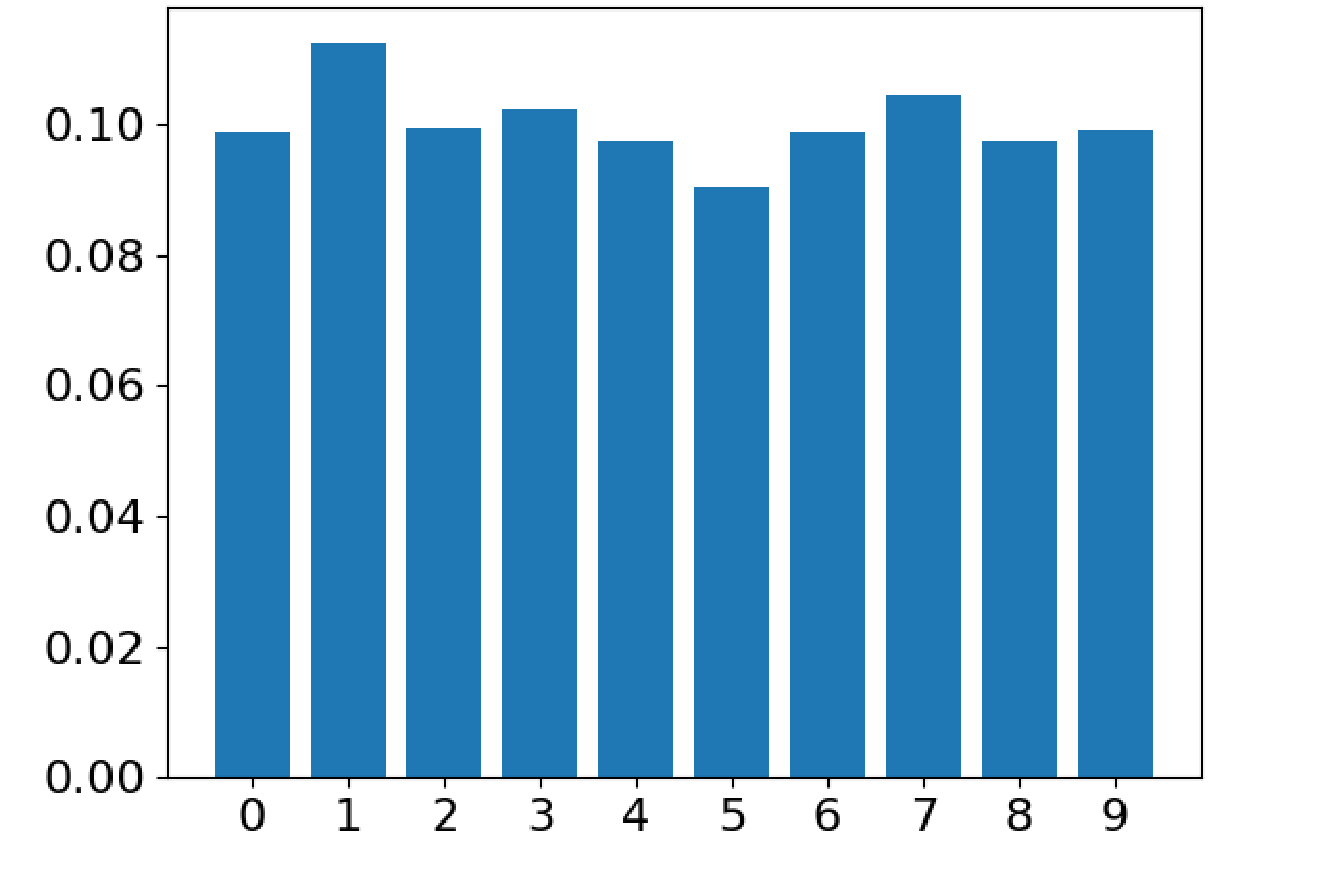
\includegraphics[width=\textwidth]{ChapterThree/mnist_dist}
		\caption{MNIST}
	\end{subfigure}
	\hfill
	\begin{subfigure}[b]{0.24\textwidth}  
		\centering 
		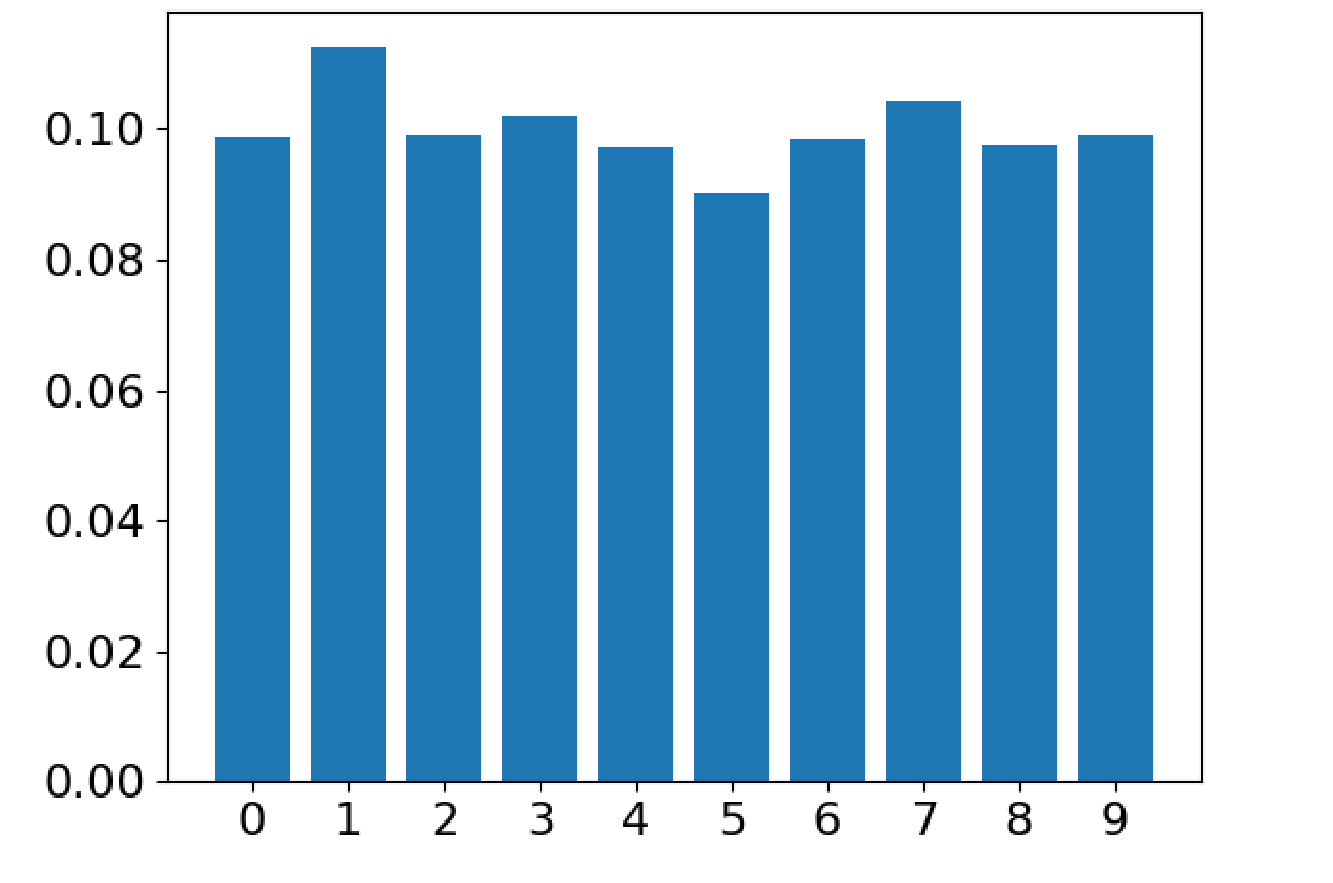
\includegraphics[width=\textwidth]{ChapterThree/mnist_m_dist}
		\caption{MNIST-M}
	\end{subfigure}
	\hfill
	\begin{subfigure}[b]{0.24\textwidth}   
		\centering 
		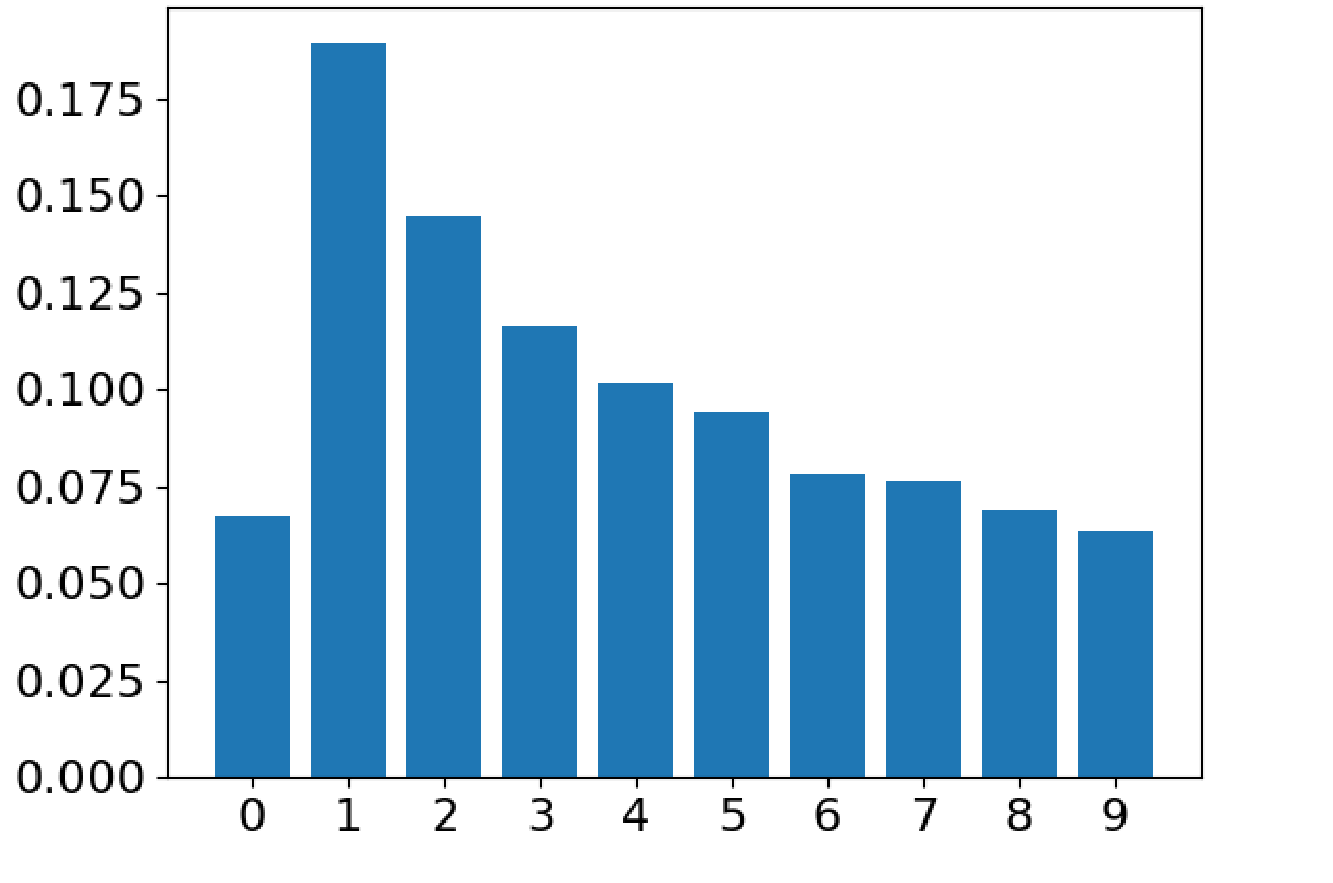
\includegraphics[width=\textwidth]{ChapterThree/svhn_dist}
		\caption{SVHN}
	\end{subfigure}
	\hfill
	\begin{subfigure}[b]{0.24\textwidth}   
		\centering 
		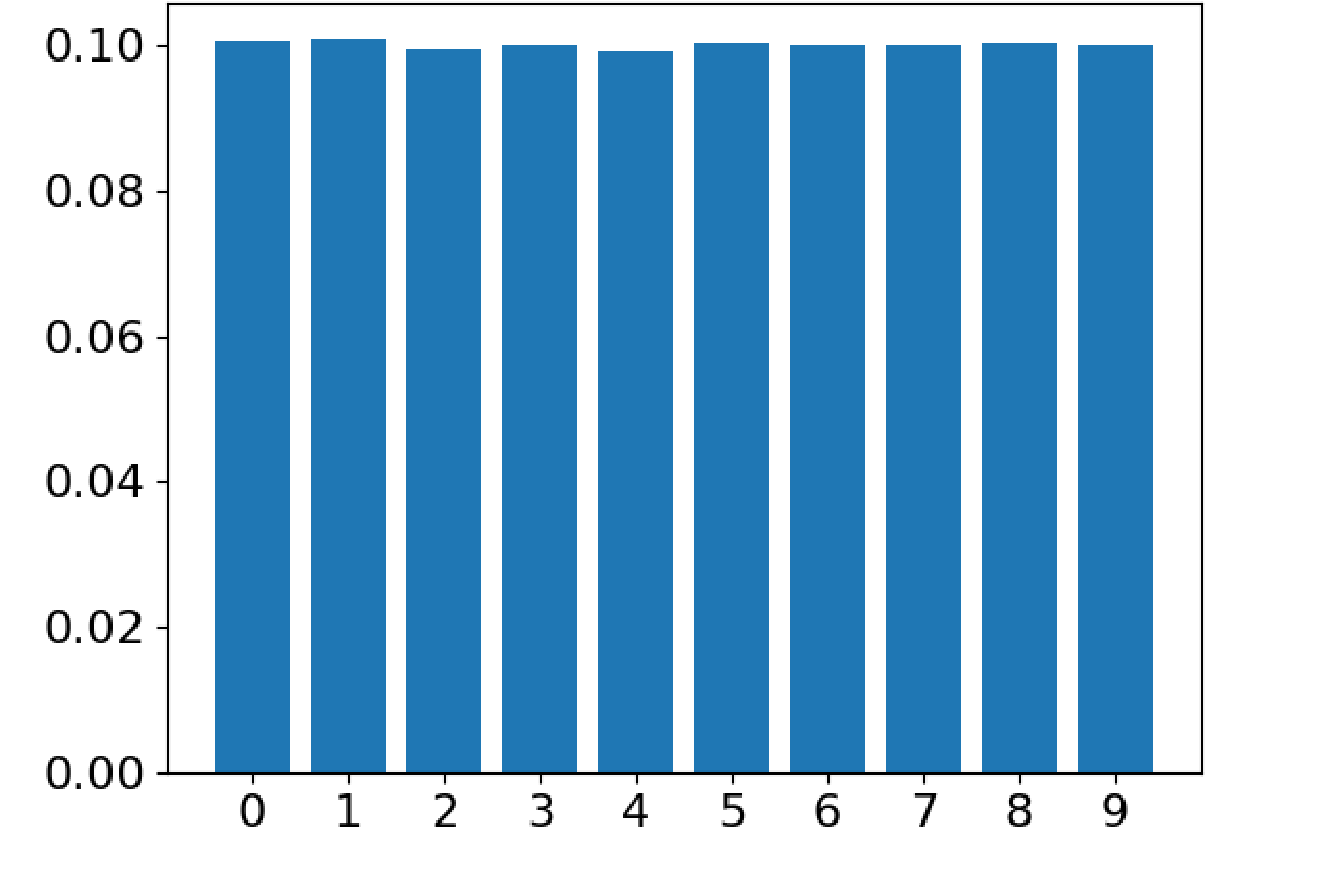
\includegraphics[width=\textwidth]{ChapterThree/synthdigits_dist}
		\caption{SynthDigits}
	\end{subfigure}
	\caption{Label distributions in the digits datasets.} 
	\label{fig:digits_dist}
\end{figure}

\begin{table}
	\centering
	\caption{Jensen-Shannon distances between the label distributions of each pair of digits domains. On each column, the largest distance is in bold and the smallest is underlined.}
	\small
	\begin{tabular}{l|cccc}
		& MNIST                & MNIST-M              & SVHN & SynthDigits \\ \hline
		MNIST       & $0$                  & $\underline{2.73 \cdot 10^{-4}}$ & $\underline{1.17 \cdot 10^{-1}}$     & $\underline{1.83 \cdot 10^{-2}}$            \\
		MNIST-M     & $\underline{2.73 \cdot 10^{-4}}$ & $0$                  & $\underline{1.17 \cdot 10^{-1}}$     & $1.84 \cdot 10^{-2}$            \\
		SVHN        & $\boldsymbol{1.17 \cdot 10^{-1}}$ & $\boldsymbol{1.17 \cdot 10^{-1}}$ & $0$                      & $\boldsymbol{1.26 \cdot 10^{-1}}$            \\
		SynthDigits & $1.83 \cdot 10^{-2}$ & $1.84 \cdot 10^{-2}$ & $\boldsymbol{1.26 \cdot 10^{-1}}$     & $0$ \\ \hline
		Average & $4.51 \cdot 10^{-2}$ &  $4.52 \cdot 10^{-2}$ & $1.20 \cdot 10^{-1}$ & $5.42 \cdot 10^{-2}$
	\end{tabular}
	\label{tab:digits_js}
\end{table}

\begin{figure}
	\centering
	\begin{subfigure}[b]{0.35\textwidth}
		\centering
		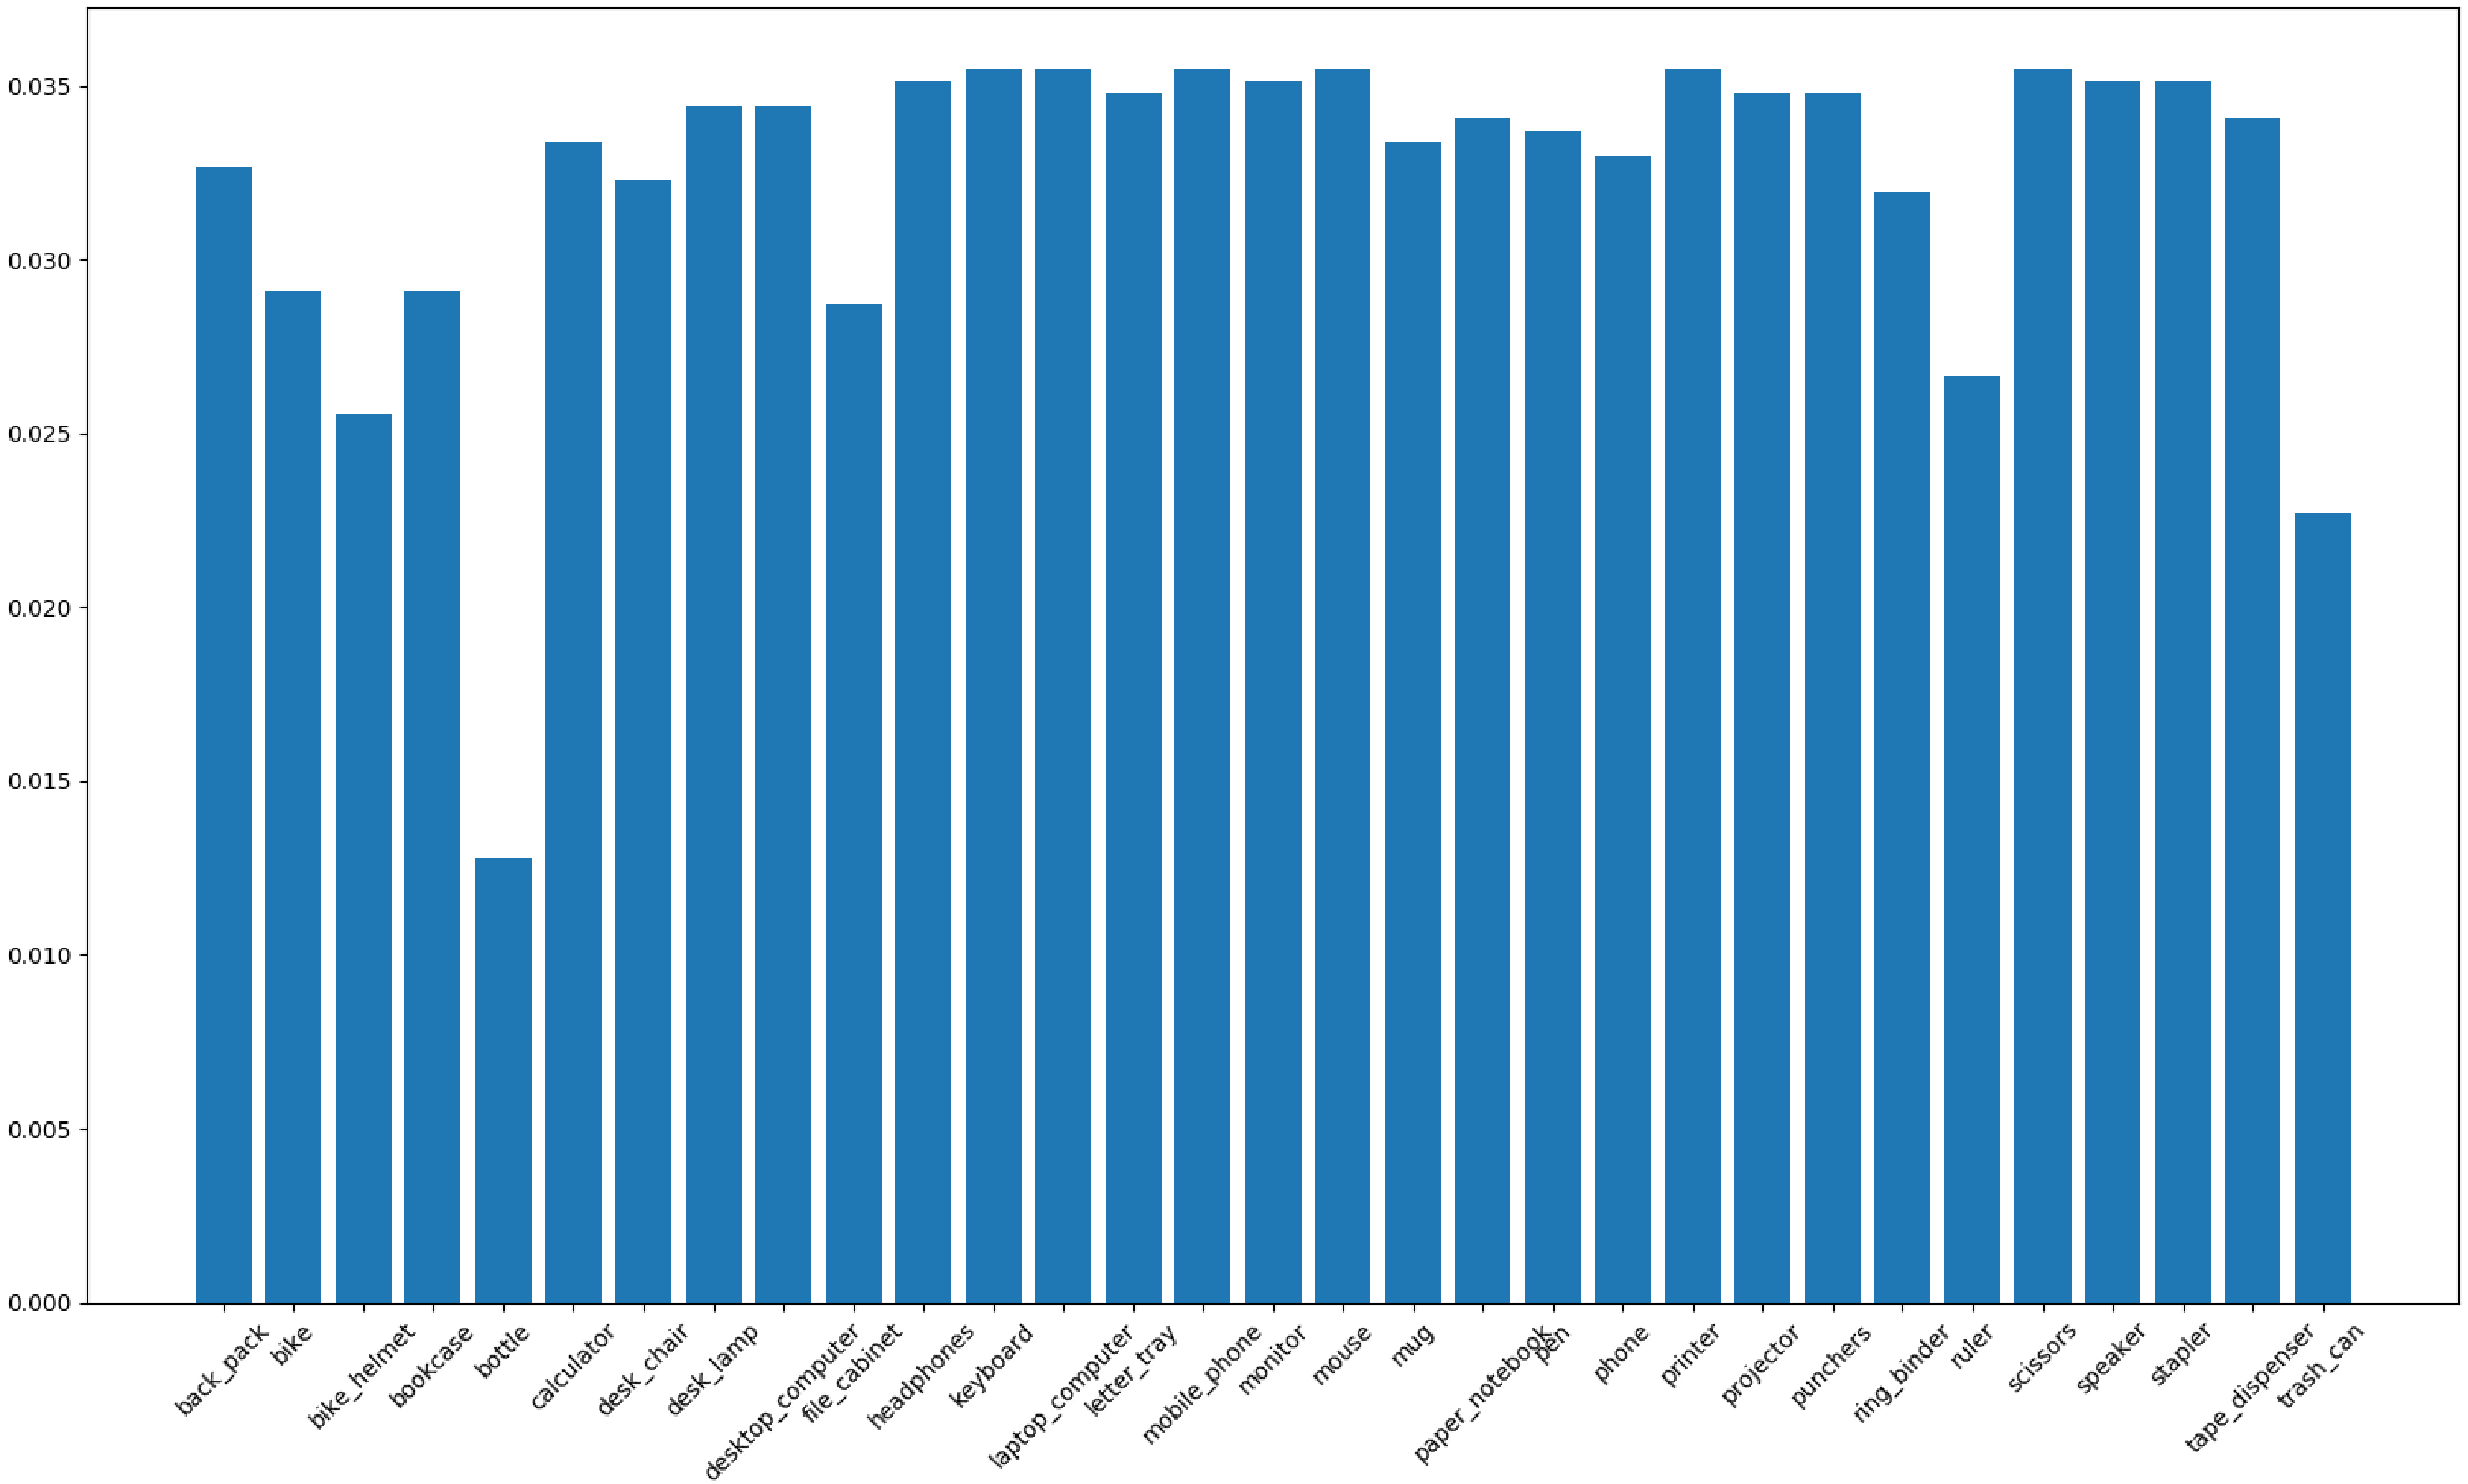
\includegraphics[width=\textwidth]{ChapterThree/amazon_dist}
		\caption{Amazon}
	\end{subfigure}
	\;%\hspace{-0.5cm}
	\begin{subfigure}[b]{0.35\textwidth}  
		\centering 
		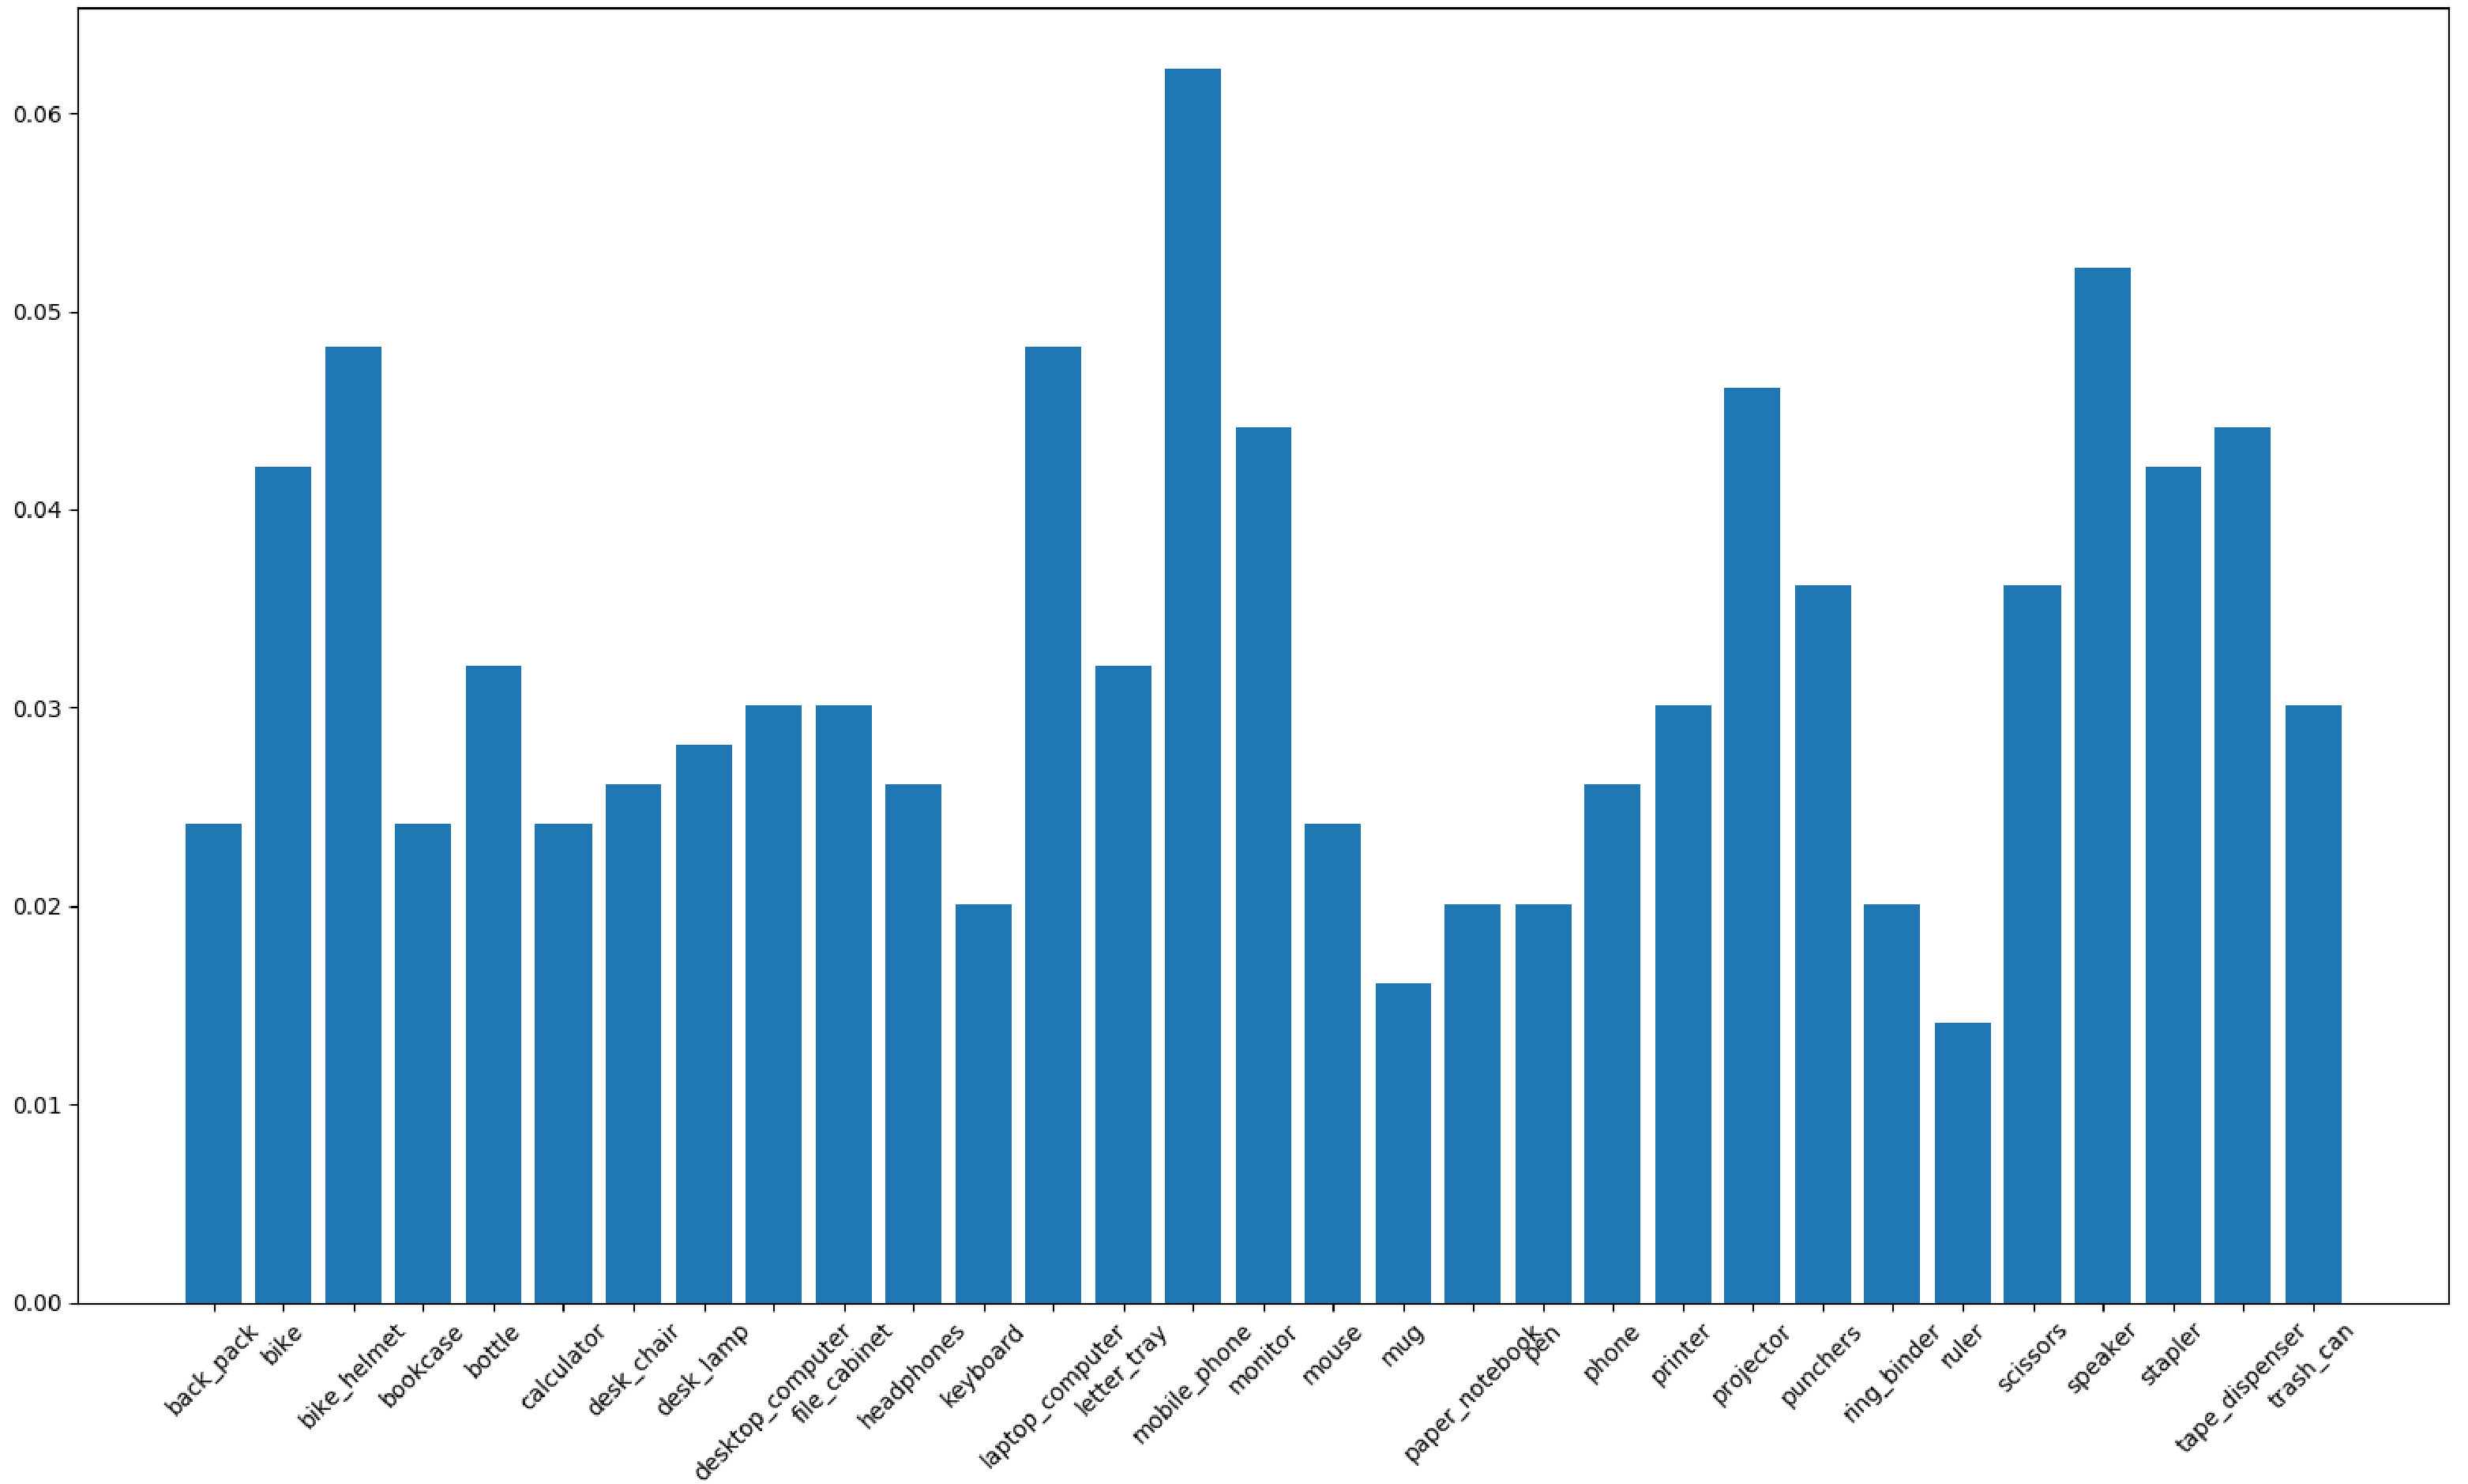
\includegraphics[width=\textwidth]{ChapterThree/dslr_dist}
		\caption{DSLR}
	\end{subfigure}
	\vskip\baselineskip
	\begin{subfigure}[b]{0.35\textwidth}   
		\centering 
		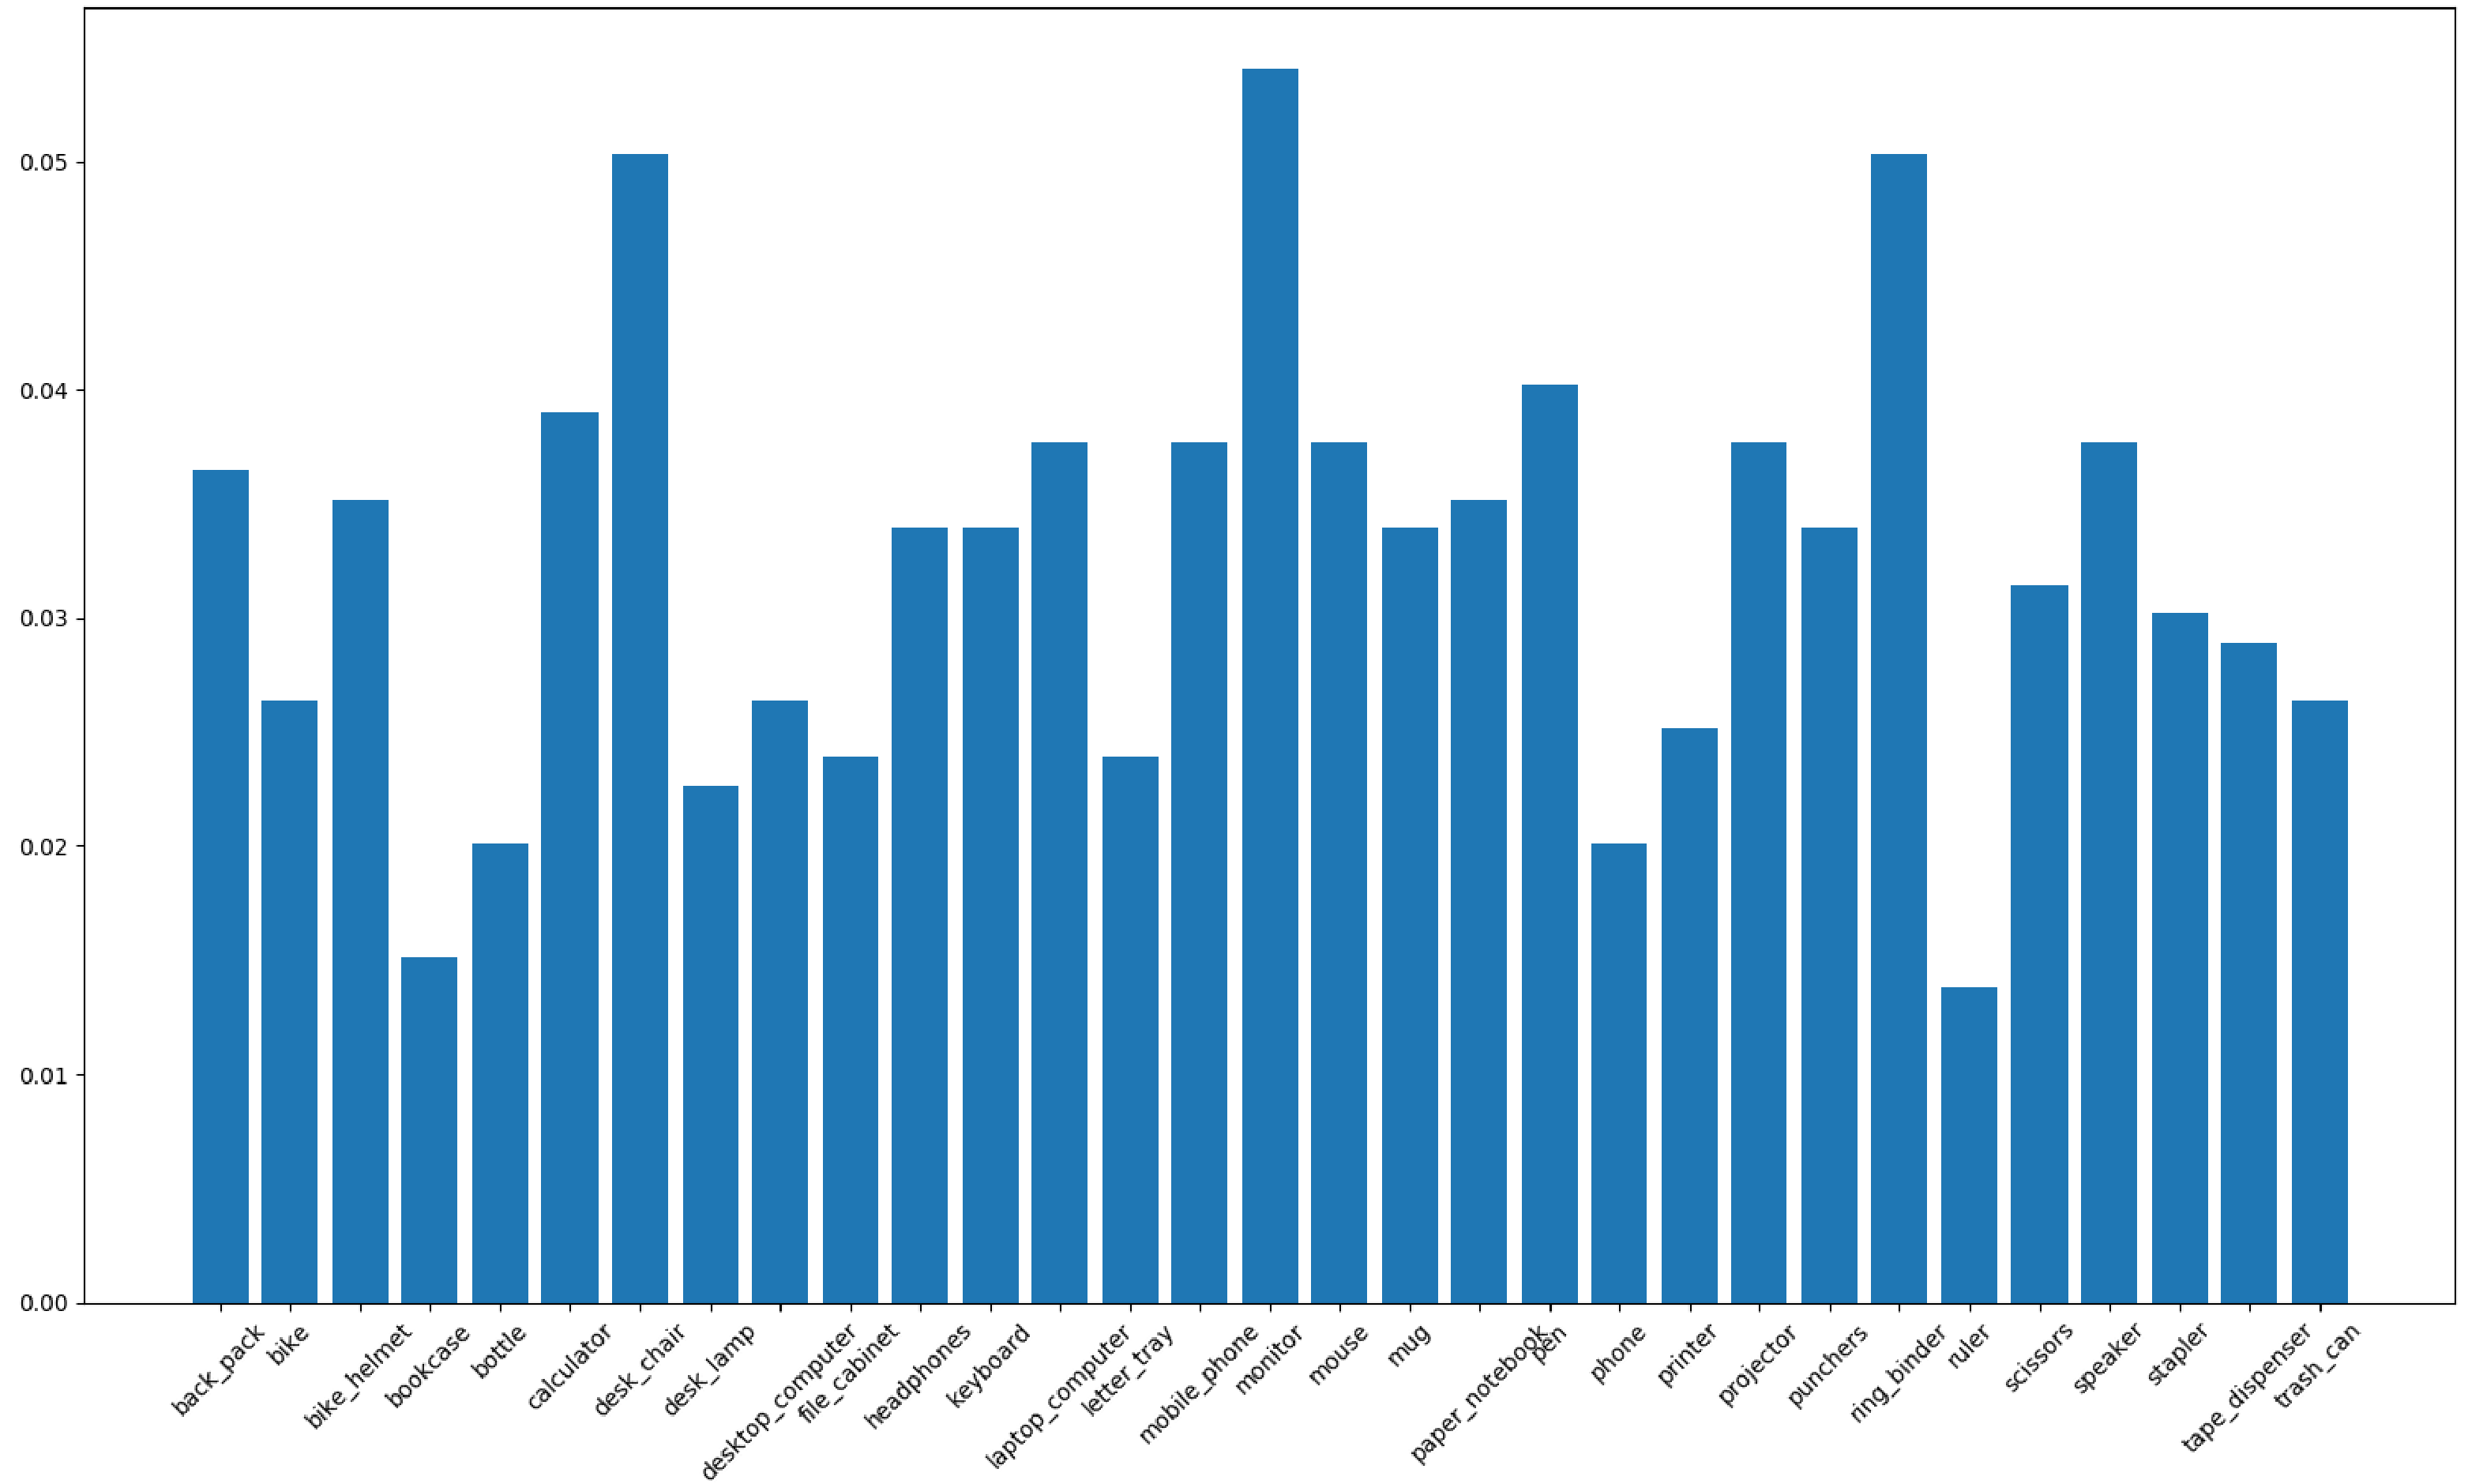
\includegraphics[width=\textwidth]{ChapterThree/webcam_dist}
		\caption{Webcam}
	\end{subfigure}
	\caption{Label distributions in Office-31.} 
	\label{fig:office_dist}
\end{figure}

\begin{table}
	\centering
	\caption{Jensen-Shannon distances between the label distributions of each pair of domains in Office-31. On each column, the largest distance is in bold.}
	\small
	\begin{tabular}{l|ccc}
		& Amazon                    & DSLR                      & Webcam                    \\ \hline
		Amazon & 0                         & $1.33 \cdot 10^{-1}$      & $9.76 \cdot 10^{-2}$      \\
		DSLR   & $\boldsymbol{1.33 \cdot 10^{-1}}$ & 0                         & $\boldsymbol{1.45 \cdot 10^{-1}}$ \\
		Webcam & $9.76 \cdot 10^{-2}$      & $\boldsymbol{1.45 \cdot 10^{-1}}$ & 0 \\ \hline
		Average & $1.15 \cdot 10^{-1}$ & $1.39 \cdot 10^{-1}$ & $1.21 \cdot 10^{-1}$
	\end{tabular}
	\label{tab:office_js}
\end{table}

\begin{figure}
	\centering
	\begin{subfigure}[b]{0.24\textwidth}
		\centering
		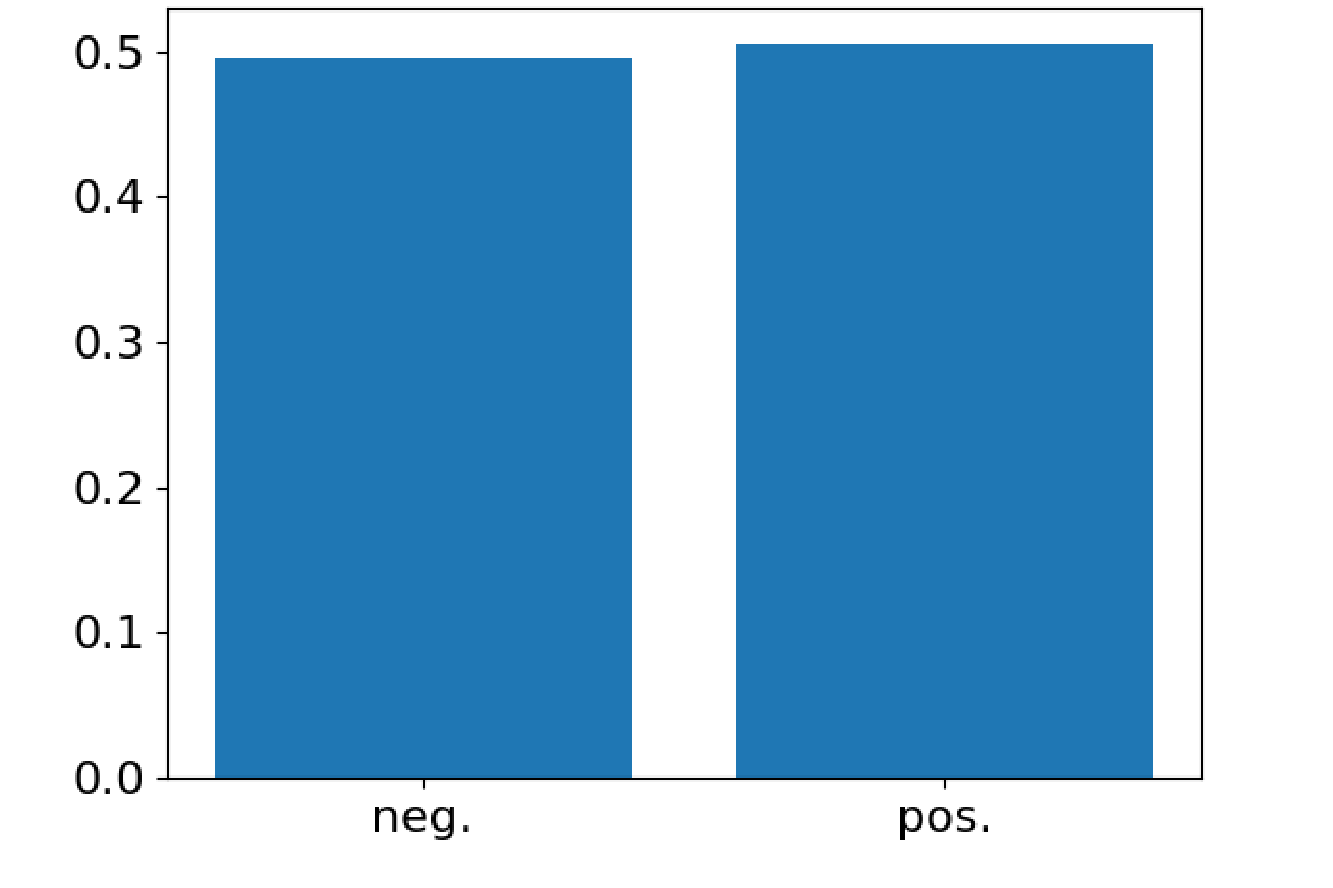
\includegraphics[width=\textwidth]{ChapterThree/books_dist}
		\caption{Books}
	\end{subfigure}
	\hfill
	\begin{subfigure}[b]{0.24\textwidth}  
		\centering 
		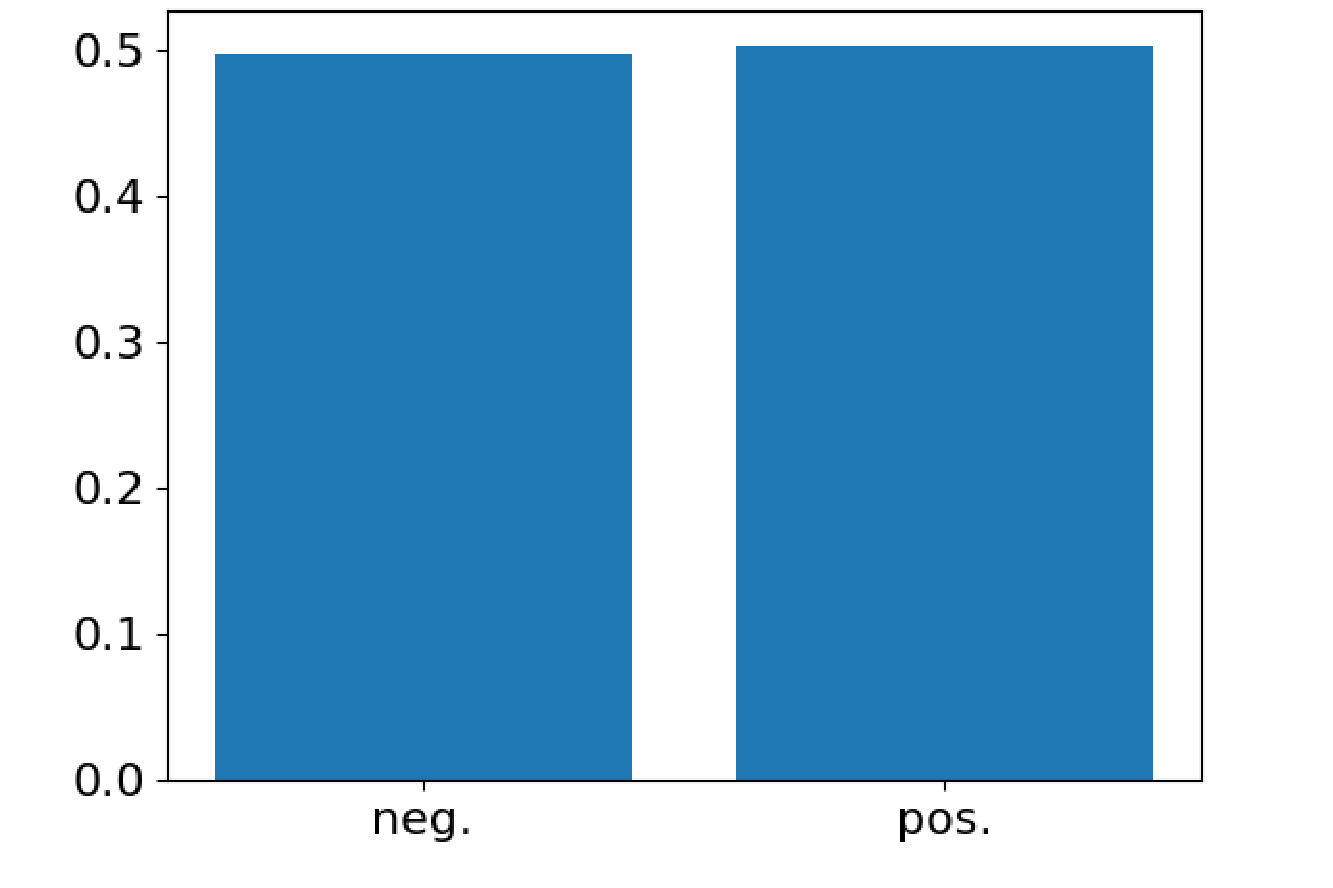
\includegraphics[width=\textwidth]{ChapterThree/dvd_dist}
		\caption{DVD}
	\end{subfigure}
	\hfill
	\begin{subfigure}[b]{0.24\textwidth}   
		\centering 
		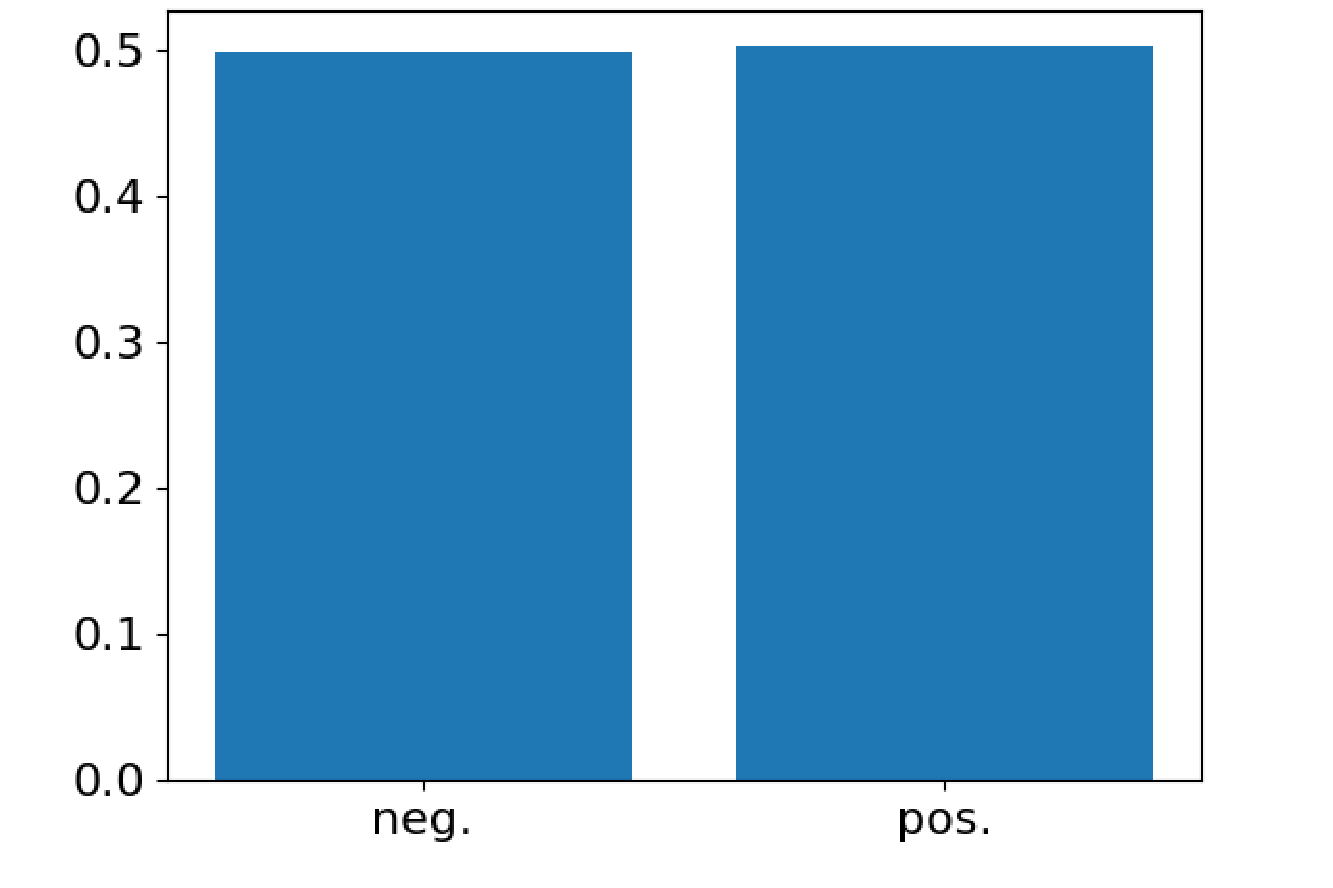
\includegraphics[width=\textwidth]{ChapterThree/electronics_dist}
		\caption{Electronics}
	\end{subfigure}
	\hfill
	\begin{subfigure}[b]{0.24\textwidth}   
		\centering 
		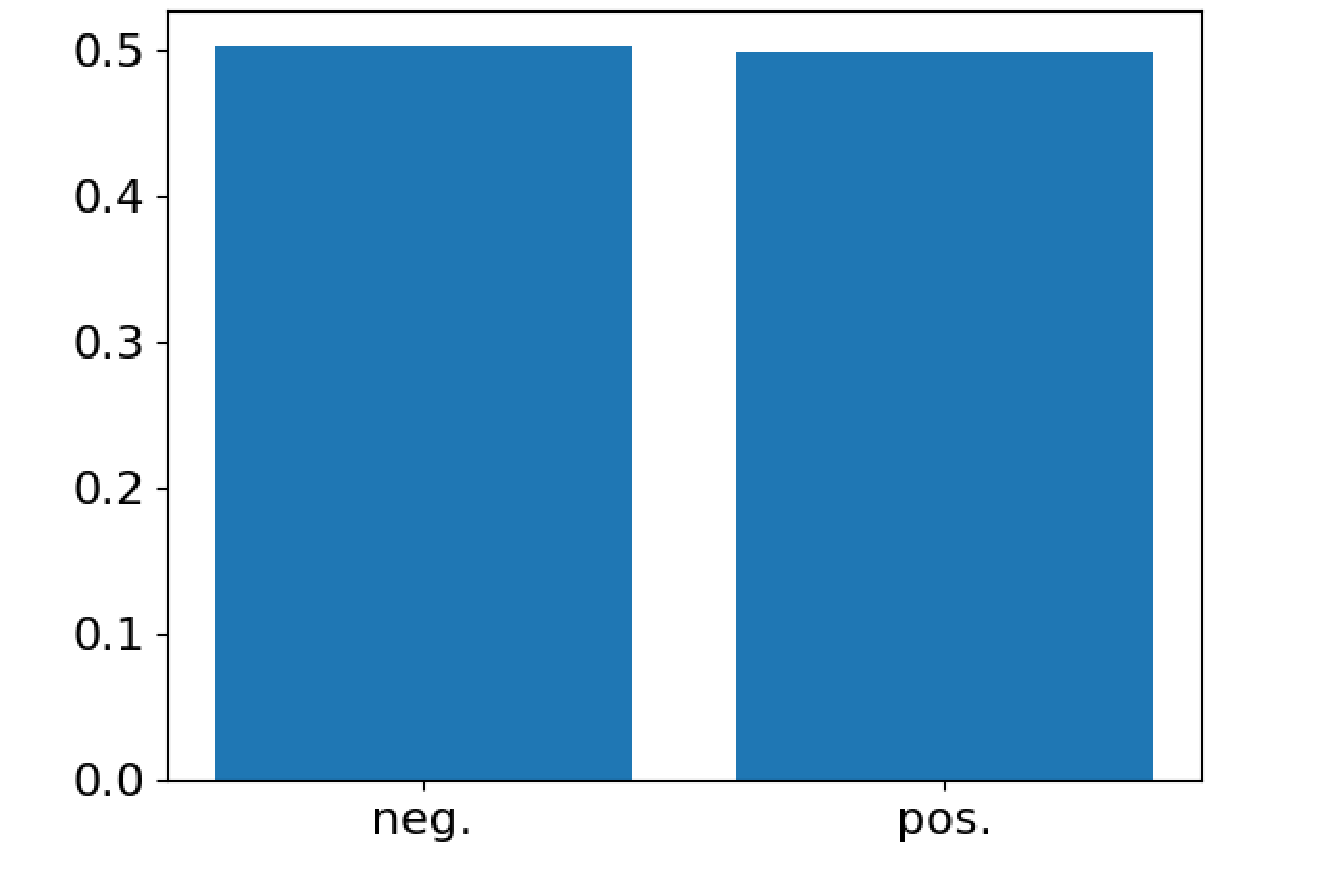
\includegraphics[width=\textwidth]{ChapterThree/kitchen_dist}
		\caption{Kitchen}
	\end{subfigure}
	\caption{Label distributions in Amazon Reviews.} 
	\label{fig:amazon_dist}
\end{figure}

\begin{table}
	\centering
	\caption{Jensen-Shannon distances between the label distributions of each pair of domains in Amazon Reviews. On each column, the largest distance is in bold and the smallest is underlined.}
	\small
	\begin{tabular}{l|cccc}
		& Books                & DVD                  & Electronics          & Kitchen              \\ \hline
		Books       & 0                    & $1.67 \cdot 10^{-3}$ & $1.93 \cdot 10^{-3}$ & $\boldsymbol{5.09 \cdot 10^{-3}}$ \\
		DVD         & $\underline{1.67 \cdot 10^{-3}}$ & 0                    & $\underline{2.53 \cdot 10^{-4}}$ & $3.42 \cdot 10^{-3}$ \\
		Electronics & $1.93 \cdot 10^{-3}$ & $\underline{2.53 \cdot 10^{-4}}$ & 0                    & $\underline{3.17 \cdot 10^{-3}}$ \\
		Kitchen     & $\boldsymbol{5.09 \cdot 10^{-3}}$ & $\boldsymbol{3.42 \cdot 10^{-3}}$ & $\boldsymbol{3.17 \cdot 10^{-3}}$ & 0 \\ \hline
		Average & $2.90 \cdot 10^{-3}$ & $1.78 \cdot 10^{-3}$ & $1.78 \cdot 10^{-3}$ & $3.89 \cdot 10^{-3}$
	\end{tabular}
	\label{tab:amazon_js}
\end{table}

\begin{table}
	\centering
	\caption{Jensen-Shannon distances between the label distributions of each pair of domains in the DomainNet dataset. On each column, the largest distance is in bold and the smallest is underlined.}
	\small
	\hspace*{-0.50in}
	\begin{tabular}{l|cccccc}
		& \textit{clp}                & \textit{inf}              & \textit{pnt} & \textit{qdr} & \textit{rel} & \textit{skt} \\ \hline
		\textit{clp} & $0$ & $3.14 \cdot 10^{-1}$ & $3.34 \cdot 10^{-1}$     & $1.98 \cdot 10^{-1}$ & $2.31 \cdot 10^{-1}$ & $2.60 \cdot 10^{-1}$         \\
		\textit{inf} & $3.14 \cdot 10^{-1}$ & $0$ & $\boldsymbol{3.79 \cdot 10^{-1}}$ & $\boldsymbol{2.83 \cdot 10^{-1}}$ & $\boldsymbol{3.03 \cdot 10^{-1}}$ & $\boldsymbol{3.26 \cdot 10^{-1}}$ \\
		\textit{pnt} & $\boldsymbol{3.34 \cdot 10^{-1}}$ & $\boldsymbol{3.79 \cdot 10^{-1}}$ & $0$ & $2.77 \cdot 10^{-1}$ & $2.99 \cdot 10^{-1}$ & $3.10 \cdot 10^{-1}$ \\
		\textit{qdr} & $\underline{1.98 \cdot 10^{-1}}$ & $\underline{2.83 \cdot 10^{-1}}$ & $\underline{2.77 \cdot 10^{-1}}$ & $0$ & $\underline{1.35 \cdot 10^{-1}}$ & $\underline{2.27 \cdot 10^{-1}}$ \\
		\textit{rel}  & $2.31 \cdot 10^{-1}$ & $3.03 \cdot 10^{-1}$ & $2.99 \cdot 10^{-1}$ & $\underline{1.35 \cdot 10^{-1}}$ & $0$ & $2.67 \cdot 10^{-1}$ \\
		\textit{skt}  & $2.60 \cdot 10^{-1}$ & $3.26 \cdot 10^{-1}$ & $3.10 \cdot 10^{-1}$ & $2.27 \cdot 10^{-1}$ & $2.67 \cdot 10^{-1}$ & $0$ \\ \hline
		Average & $2.67 \cdot 10^{-1}$ & $3.21 \cdot 10^{-1}$ & $3.20 \cdot 10^{-1}$ & $2.24 \cdot 10^{-1}$ & $2.47 \cdot 10^{-1}$ & $2.78 \cdot 10^{-1}$ \\
	\end{tabular}
	\label{tab:domainnet_js}
\end{table}

\subsection{Effect of over-training}
\label{sec:overtrain}
When the label distributions differ across domains, training the feature extractor and domain discriminator for a large number of iterations tends to lead to an increased target error. This is a direct effect of the curse of domain-invariant representations and it has been verified experimentally in \cite{Zhao2019}.

In this experiment, we want to evaluate if the increased robustness of the feature extractor provided by the adopted consistency regularization helps to mitigate this issue. For this purpose, we use Office-31 since it is fairly small and therefore easy to overtrain and the label distributions across domains are significantly skewed (see \ref{sec:label_dist}). We train our model and two baselines (MDAN~\citep{Zhao2018} and MODA) for 60 epochs and we observe the evolution of the model accuracy on the target data. The plots are shown in \Figref{fig:overtrain}. As we see there, in MODA-FM the accuracy keeps stable after reaching the maximum in all domains. Contrarily, in MODA and especially in MDAN, the accuracy tends to decay after reaching the maximum. These observations strongly suggest that MODA-FM succeeds on mitigating the curse of domain-invariant representations. In MODA the problem is less pronounced than in MDAN probably because the latter will continue optimizing itself until it can produce domain-invariant representations for all source domains, whereas the former will simply ignore the hardest source domains by assigning them a low weight (possibly even zero).

\begin{figure}
	\centering
	\hspace*{-0.30in}
	\begin{subfigure}[b]{0.32\textwidth}
		\begin{tikzpicture}[scale=0.58, every node/.style={scale=0.58}]
		\begin{axis}[
		enlargelimits=false,
		legend style={at={(0.45,0.1)},anchor=south west,font=\large},
		xlabel=\huge epoch, xmin=0, xmax=60, xtick={0,10,20,30,40,50,60},
		ylabel=\huge accuracy, ymin=0.55, ymax=0.75, ytick={0.55,0.6,0.65,0.7,0.75},
		grid=both, grid style={line width=.1pt, draw=gray!10},
		]   
		\addplot[color=myblue,smooth,thick]table[x=Epoch, y=MDAN, col sep=comma]{Figures/ChapterThree/amazon_long.txt};
		\addlegendentry{MDAN ($\pgfmathprintnumber{\slopeMDAN}$)}
		
		\addplot[color=myorange,smooth,thick]table[x=Epoch, y=MixMDAN, col sep=comma]{Figures/ChapterThree/amazon_long.txt};
		\addlegendentry{MODA ($\pgfmathprintnumber{\slopeMODA}$)}
		
		\addplot[color=mygreen,smooth,thick]table[x=Epoch, y=Ours, col sep=comma]{Figures/ChapterThree/amazon_long.txt};
		\addlegendentry{MODA-FM ($\pgfmathprintnumber{\slopeMODAFM}$)}
		
		\addplot[color=gray,dashed] table [col sep = comma,y={create col/linear regression={y=1}},skip first n=2]{Figures/ChapterThree/amazon_long.txt};
		\xdef\slopeMDAN{\pgfplotstableregressiona}
		\addplot[color=gray,dashed] table [col sep = comma,y={create col/linear regression={y=2}},skip first n=2]{Figures/ChapterThree/amazon_long.txt};
		\xdef\slopeMODA{\pgfplotstableregressiona}
		\addplot[color=gray,dashed] table [col sep = comma,y={create col/linear regression={y=3}},skip first n=2]{Figures/ChapterThree/amazon_long.txt};
		\xdef\slopeMODAFM{\pgfplotstableregressiona}
		\end{axis}
		\end{tikzpicture}
		\caption{Amazon}
	\end{subfigure}
	\hfill%
	\begin{subfigure}[b]{0.32\textwidth}
		\centering
		\hspace*{-0.30in}
		\begin{tikzpicture}[scale=0.58, every node/.style={scale=0.58}]
		\begin{axis}[
		enlargelimits=false,
		legend style={at={(0.45,0.1)},anchor=south west,font=\large},
		xlabel=\huge epoch, xmin=0, xmax=60, xtick={0,10,20,30,40,50,60},
		ylabel=\huge accuracy, ymin=0.8, ymax=1, ytick={0.8,0.85,0.9,0.95,1},
		grid=both, grid style={line width=.1pt, draw=gray!10},
		]   
		\addplot[color=myblue,smooth,thick]table[x=Epoch, y=MDAN, col sep=comma]{Figures/ChapterThree/dslr_long.txt};
		\addlegendentry{MDAN ($\pgfmathprintnumber{\slopeMDAN}$)}
		
		\addplot[color=myorange,smooth,thick]table[x=Epoch, y=MixMDAN, col sep=comma]{Figures/ChapterThree/dslr_long.txt};
		\addlegendentry{MODA ($\pgfmathprintnumber{\slopeMODA}$)}
		
		\addplot[color=mygreen,smooth,thick]table[x=Epoch, y=Ours, col sep=comma]{Figures/ChapterThree/dslr_long.txt};
		\addlegendentry{MODA-FM ($\pgfmathprintnumber{\slopeMODAFM}$)}
		
		\addplot[color=gray,dashed] table [col sep = comma,y={create col/linear regression={y=1}},skip first n=2]{Figures/ChapterThree/dslr_long.txt};
		\xdef\slopeMDAN{\pgfplotstableregressiona}
		\addplot[color=gray,dashed] table [col sep = comma,y={create col/linear regression={y=2}},skip first n=2]{Figures/ChapterThree/dslr_long.txt};
		\xdef\slopeMODA{\pgfplotstableregressiona}
		\addplot[color=gray,dashed] table [col sep = comma,y={create col/linear regression={y=3}},skip first n=2]{Figures/ChapterThree/dslr_long.txt};
		\xdef\slopeMODAFM{\pgfplotstableregressiona}
		\end{axis}
		\end{tikzpicture}
		\caption{DSLR}
	\end{subfigure}
	\hfill%
	\begin{subfigure}[b]{0.32\textwidth}
		\centering
		\hspace*{-0.30in}
		\begin{tikzpicture}[scale=0.58, every node/.style={scale=0.58}]
		\begin{axis}[
		enlargelimits=false,
		legend style={at={(0.45,0.1)},anchor=south west,font=\large},
		xlabel=\huge epoch, xmin=0, xmax=60, xtick={0,10,20,30,40,50,60},
		ylabel=\huge accuracy, ymin=0.8, ymax=1, ytick={0.8,0.85,0.9,0.95,1},
		grid=both, grid style={line width=.1pt, draw=gray!10},
		]   
		\addplot[color=myblue,smooth,thick]table[x=Epoch, y=MDAN, col sep=comma]{Figures/ChapterThree/webcam_long.txt};
		\addlegendentry{MDAN ($\pgfmathprintnumber{\slopeMDAN}$)}
		
		\addplot[color=myorange,smooth,thick]table[x=Epoch, y=MixMDAN, col sep=comma]{Figures/ChapterThree/webcam_long.txt};
		\addlegendentry{MODA ($\pgfmathprintnumber{\slopeMODA}$)}
		
		\addplot[color=mygreen,smooth,thick]table[x=Epoch, y=Ours, col sep=comma]{Figures/ChapterThree/webcam_long.txt};
		\addlegendentry{MODA-FM ($\pgfmathprintnumber{\slopeMODAFM}$)}
		
		\addplot[color=gray,dashed] table [col sep = comma,y={create col/linear regression={y=1}},skip first n=2]{Figures/ChapterThree/webcam_long.txt};
		\xdef\slopeMDAN{\pgfplotstableregressiona}
		\addplot[color=gray,dashed] table [col sep = comma,y={create col/linear regression={y=2}},skip first n=2]{Figures/ChapterThree/webcam_long.txt};
		\xdef\slopeMODA{\pgfplotstableregressiona}
		\addplot[color=gray,dashed] table [col sep = comma,y={create col/linear regression={y=3}},skip first n=2]{Figures/ChapterThree/webcam_long.txt};
		\xdef\slopeMODAFM{\pgfplotstableregressiona}
		\end{axis}
		\end{tikzpicture}
		\caption{Webcam}
	\end{subfigure}
	\caption{Test accuracy along 60 training epochs for our model and two baselines in Office-31. The tendency line for each curve is also shown (dashed lines) and the respective slope is indicated in brackets in each plot legend. The domain indicated below each plot is the target.}
	\label{fig:overtrain}
\end{figure}

\subsection{Hyperparameter sensitivity analysis}
\label{sec:hyperparam}
Our model comprises three main hyperparameters: $\mu_d$, $\mu_s$ and $\mu_c$. The hyperparameter $\mu_d$ controls the relative weight of the domain discriminator loss and is present in every work on adversarial DA, thus its effect has already been studied extensively. For this reason, we focus on the effect of $\mu_s$ and $\mu_c$. We use the digits datasets and evaluate the accuracy on each target domain while varying either $\mu_s$ or $\mu_c$ and keeping the other one constant at the optimal value.

A sufficiently large value of $\mu_s$ forces $\alpha$ to converge to a vector with all components equal to $1/M$, weighting all source domains equally. Setting $\mu_s$ close to zero corresponds to the most optimistic scenario: the sparsity penalization is dropped and so, after sufficiently many training iterations, $\alpha$ would converge to a one-hot vector, choosing the source domain with the minimum difference of classification and discrimination losses ($\gL_{class} - \mu_d\gL_{disc}$). \Figref{fig:hyperparam_mu_s} shows that, for MNIST, similar results are obtained with any of those strategies. The fact that digits classification in MNIST is significantly easier than in any of the remaining datasets likely explains this behavior. Domain adaptation for MNIST-M is slightly favored by smaller values of $\mu_s$, meaning that a more optimistic approach works better here. For SVHN, the opposite holds and the results are very poor when low sparsity regularization is employed. There is even a strong discontinuity in the accuracy plot for this domain around $\mu_s \approx 0.2$. This discontinuity divides situations where $\alpha$ collapses into the easiest source domain ($\mu_s < 0.2$) and those where it does not collapse ($\mu_s > 0.2$). We elaborate more on this in \ref{sec:alpha_evol}. In all cases, we observe that a $\mu_s \in [0.2, 0.6]$ provides near-optimal results.

The effect of varying $\mu_c$ is plotted in \Figref{fig:hyperparam_mu_c}. Values of $\mu_c$ close to zero drop the consistency regularization and, therefore, we obtain results close to those of MODA. Significant performance gains are obtained for $\mu_c > 0.01$ and the optimal is reached for $\mu_c \in [0.4, 1.0]$ for all domains.

\begin{figure}
	\centering
	\hspace*{-0.30in}
	\begin{subfigure}[b]{0.45\textwidth}
		\centering
		\begin{tikzpicture}[scale=0.8, every node/.style={scale=0.58}]
		\begin{semilogxaxis}[xmin=5e-5, xmax=50, ymin=0, ymax=1.05, domain=1e-5:20, ylabel=\large accuracy,
		scaled x ticks=real:1e-3,
		xtick scale label code/.code={},
		log x ticks with fixed point/.style={
			xticklabel={
				\pgfkeys{/pgf/fpu=true}
				\pgfmathparse{exp(\tick)}%
				\pgfmathprintnumber[fixed relative, precision=3]{\pgfmathresult}
				\pgfkeys{/pgf/fpu=false}
			}
		},
		legend style={at={(0.65,0.1)},anchor=south west,font=\normalsize},
		grid=both, grid style={line width=.1pt, draw=gray!10}]
		
		\addplot[color=myblue,only marks,sharp plot,mark=*]table[x index={0}, y index={1}, col sep=comma, skip first n=2]{Figures/ChapterThree/mu_s.txt};
		\addlegendentry{MNIST}
		
		\addplot[color=myorange,only marks,sharp plot,mark=*]table[x index={0}, y index={2}, col sep=comma, skip first n=2]{Figures/ChapterThree/mu_s.txt};
		\addlegendentry{MNIST-M}
		
		\addplot[color=mygreen,only marks,sharp plot,mark=*]table[x index={0}, y index={3}, col sep=comma, skip first n=2]{Figures/ChapterThree/mu_s.txt};
		\addlegendentry{SVHN}
		\end{semilogxaxis}
		\end{tikzpicture}
		\caption{$\mu_s$}
		\label{fig:hyperparam_mu_s}
	\end{subfigure}
	\hfill%
	\begin{subfigure}[b]{0.45\textwidth}
		\centering
		\begin{tikzpicture}[scale=0.8, every node/.style={scale=0.58}]
		\begin{semilogxaxis}[xmin=5e-5, xmax=50, ymin=0, ymax=1.05, domain=1e-5:20, ylabel=\large accuracy,
		scaled x ticks=real:1e-3,
		xtick scale label code/.code={},
		log x ticks with fixed point/.style={
			xticklabel={
				\pgfkeys{/pgf/fpu=true}
				\pgfmathparse{exp(\tick)}%
				\pgfmathprintnumber[fixed relative, precision=3]{\pgfmathresult}
				\pgfkeys{/pgf/fpu=false}
			}
		},
		legend style={at={(0.65,0.1)},anchor=south west,font=\normalsize},
		grid=both, grid style={line width=.1pt, draw=gray!10}]
		
		\addplot[color=myblue,only marks,sharp plot,mark=*]table[x index={0}, y index={1}, col sep=comma, skip first n=2]{Figures/ChapterThree/mu_c.txt};
		\addlegendentry{MNIST}
		
		\addplot[color=myorange,only marks,sharp plot,mark=*]table[x index={0}, y index={2}, col sep=comma, skip first n=2]{Figures/ChapterThree/mu_c.txt};
		\addlegendentry{MNIST-M}
		
		\addplot[color=mygreen,only marks,sharp plot,mark=*]table[x index={0}, y index={3}, col sep=comma, skip first n=2]{Figures/ChapterThree/mu_c.txt};
		\addlegendentry{SVHN}
		\end{semilogxaxis}
		\end{tikzpicture}
		\caption{$\mu_c$}
		\label{fig:hyperparam_mu_c}
	\end{subfigure}
	\caption{Test accuracy as a function of hyperparameters $\mu_s$ (a) and $\mu_c$ (b) using the digits datasets. The domain corresponding to each line is the target.}
	\label{fig:hyperparam}
\end{figure}

\subsection{Evolution of the source weights}
\label{sec:alpha_evol}
Here, we study the evolution of the source weights $\alpha$ along training. The behavior is determined by the evolution of the classification and discrimination losses of each source domain and also by the choice of the hyperparameter $\mu_s$. The effect of varying $\mu_s$ on the model performance was analyzed in \ref{sec:hyperparam}. Now, we are interested in observing the dynamics of $\alpha$ along the training epochs, for different source domains, using the corresponding optimal $\mu_s$. We use the digits datasets for this purpose and we present the results in \Figref{fig:alpha_train}.

For MNIST, where the lowest $\mu_s$ is used, we observe that the mixture coefficients rapidly collapse into the easiest source domain (SynthDigits). Nonetheless, in \ref{sec:hyperparam} we have observed that the target accuracy for MNIST was almost insensitive to the choice of $\mu_s$, meaning that using only the data from the easiest source domain or weighting all source domains equally would produce identical results. When we take MNIST-M and SVHN as target domains, with a slightly increased $\mu_s$, a different behavior occurs. Early in the training process, the weight for the easiest source domain (MNIST) increases rapidly, following the fast decrease in the corresponding loss. Later, as the loss for the easiest source domain plateaus and the remaining keep decreasing, the  weights for the remaining active source domains start to increase. This behavior explains the discontinuity we have observed in the plot of target accuracy vs. $\mu_s$ for SVHN (\Figref{fig:hyperparam_mu_s}): if $\mu_s$ is sufficiently small to allow $\alpha$ to rapidly collapse into MNIST, the data of the remaining source domains is simply discarded for the remaining of the training process and the corresponding weights will never increase.

\begin{figure}
	\centering
	\hspace*{-0.50in}
	\begin{subfigure}[b]{0.32\textwidth}
		\begin{tikzpicture}[scale=0.58, every node/.style={scale=0.58}]
		\begin{axis}[
		enlargelimits=false,
		legend style={at={(0.65,0.1)},anchor=south west,font=\large},
		xlabel=\huge epoch, xmin=0, xmax=60, xtick={0,10,20,30,40,50,60},
		ylabel=\huge $\alpha$, ymin=0., ymax=1., 
		grid=both, grid style={line width=.1pt, draw=gray!10},
		title=\text{\huge $\mu_s=0.1$}
		]   
		\addplot[color=myorange,smooth,thick]table[x=Epoch, y=MNIST_M, col sep=comma]{Figures/ChapterThree/mnist_coef.txt};
		\addlegendentry{MNIST-M}
		
		\addplot[color=mygreen,smooth,thick]table[x=Epoch, y=SVHN, col sep=comma]{Figures/ChapterThree/mnist_coef.txt};
		\addlegendentry{SVHN}
		
		\addplot[color=myred,smooth,thick]table[x=Epoch, y=SynthDigits, col sep=comma]{Figures/ChapterThree/mnist_coef.txt};
		\addlegendentry{SynthDigits}
		\end{axis}
		\end{tikzpicture}
		\caption{MNIST}
	\end{subfigure}
	\hfill%
	\begin{subfigure}[b]{0.32\textwidth}
		\centering
		\begin{tikzpicture}[scale=0.58, every node/.style={scale=0.58}]
		\begin{axis}[
		enlargelimits=false,
		legend style={at={(0.65,0.1)},anchor=south west,font=\large},
		xlabel=\huge epoch, xmin=0, xmax=60, xtick={0,10,20,30,40,50,60},
		ylabel=\huge $\alpha$, ymin=0., ymax=1.,
		grid=both, grid style={line width=.1pt, draw=gray!10},
		title=\text{\huge$\mu_s=0.2$}
		]   
		\addplot[color=myblue,smooth,thick]table[x=Epoch, y=MNIST, col sep=comma]{Figures/ChapterThree/mnist_m_coef.txt};
		\addlegendentry{MNIST}
		
		\addplot[color=mygreen,smooth,thick]table[x=Epoch, y=SVHN, col sep=comma]{Figures/ChapterThree/mnist_m_coef.txt};
		\addlegendentry{SVHN}
		
		\addplot[color=myred,smooth,thick]table[x=Epoch, y=SynthDigits, col sep=comma]{Figures/ChapterThree/mnist_m_coef.txt};
		\addlegendentry{SynthDigits}
		\end{axis}
		\end{tikzpicture}
		\caption{MNIST-M}
	\end{subfigure}
	\hfill%
	\begin{subfigure}[b]{0.32\textwidth}
		\centering
		\begin{tikzpicture}[scale=0.58, every node/.style={scale=0.58}]
		\begin{axis}[
		enlargelimits=false,
		legend style={at={(0.65,0.1)},anchor=south west,font=\large},
		xlabel=\huge epoch, xmin=0, xmax=60, xtick={0,10,20,30,40,50,60},
		ylabel=\huge $\alpha$, ymin=0., ymax=1,
		grid=both, grid style={line width=.1pt, draw=gray!10},
		title=\text{\huge$\mu_s=0.9$}
		]   
		\addplot[color=myblue,smooth,thick]table[x=Epoch, y=MNIST, col sep=comma]{Figures/ChapterThree/svhn_coef.txt};
		\addlegendentry{MNIST}
		
		\addplot[color=myorange,smooth,thick]table[x=Epoch, y=MNIST_M, col sep=comma]{Figures/ChapterThree/svhn_coef.txt};
		\addlegendentry{MNIST-M}
		
		\addplot[color=myred,smooth,thick]table[x=Epoch, y=SynthDigits, col sep=comma]{Figures/ChapterThree/svhn_coef.txt};
		\addlegendentry{SynthDigits}
		\end{axis}
		\end{tikzpicture}
		\caption{SVHN}
	\end{subfigure}
	\caption{Source weights $\alpha$ for each domain along 60 training epochs in the digits datasets. The target domain and the value of $\mu_s$ that was used are indicated below and above each plot, respectively.}
	\label{fig:alpha_train}
\end{figure}

\subsection{Network architectures}
\label{sec:arch}
The following notation is used to designate network layers: \texttt{Conv(n, k)} -- 2-D convolutional layer with \texttt{n} output channels, square kernels with size \texttt{k}, and unit stride, followed by a rectified linear activation; \texttt{MaxPool(k)} -- 2-D max-pooling over non-overlapping regions of $\texttt{k} \times \texttt{k}$ pixels; \texttt{AdaptAvgPool(k)} -- 2-D adaptive average pooling where the output size is $\texttt{k} \times \texttt{k}$ pixels. \texttt{FC(n)} -- fully-connected layer with $\texttt{n}$ output neurons, followed by a rectified linear activation except for output layers; \texttt{Dropout(p)} -- dropout layer where $\texttt{p}$ is the probability of zeroing an element. A gradient reversal layer~\citep{Ganin2015} is present at the input of the domain discriminator in all models. All classifiers and domain discriminators are followed by a softmax layer that maps the output to the corresponding class probabilities.

\paragraph{Digits classification} Input images have shape $3 \times 32 \times 32$. Feature extractor: \texttt{Conv(64, 3)}~$\rightarrow$ \texttt{MaxPool(2)}~$\rightarrow$ \texttt{Conv(128, 3)}~$\rightarrow$ \texttt{MaxPool(2)}~$\rightarrow$ \texttt{Conv(256, 3)}. Task classifier: \texttt{MaxPool(2)}~$\rightarrow$ \texttt{Conv(256, 3)}~$\rightarrow$ \texttt{FC(2048)}~$\rightarrow$ \texttt{FC(1024)}~$\rightarrow$ \texttt{FC(10)}. Domain discriminator: \texttt{MaxPool(2)}~$\rightarrow$ \texttt{FC(2048)}~$\rightarrow$ \texttt{FC(2048)}~$\rightarrow$ \texttt{FC(1024)}~$\rightarrow$ \texttt{FC(2)}.

\paragraph{Object classification (Office-31 dataset)} Input images have shape $3 \times 256 \times 256$. Feature extractor: ResNet-50 up to stage~3. Task classifier / domain discriminator: ResNet-50 stage~4~$\rightarrow$ \texttt{AdaptAvgPool(1)}~$\rightarrow$ \texttt{FC(\#classes)}, where $\texttt{\#classes} = 31$ for the task classifier and $\texttt{\#classes} = 2$ for the domain discriminator.

\paragraph{Sentiment analysis (Amazon Reviews dataset)} Input features have dimension $5000$. Feature extractor: \texttt{Dropout(p)}~$\rightarrow$ \texttt{FC(1000)}~$\rightarrow$ \texttt{Dropout(p)}~$\rightarrow$ \texttt{FC(500)}~$\rightarrow$ \texttt{Dropout(p)}~$\rightarrow$ \texttt{FC(100)}~$\rightarrow$ \texttt{Dropout(p)}, where $\texttt{p} = 0$ except for producing the augmented samples used in the consistency regularization. Task classifier / domain discriminator: \texttt{FC(2)}.

\paragraph{Large scale object classification (DomainNet dataset)} Input images have shape $3 \times 192 \times 192$. Feature extractor: ResNet-152 up to stage~3. Task classifier / domain discriminator: ResNet-152 stage~4~$\rightarrow$ \texttt{AdaptAvgPool(1)}~$\rightarrow$ \texttt{FC(\#classes)}, where $\texttt{\#classes} = 345$ for the task classifier and $\texttt{\#classes} = 2$ for the domain discriminator.

\subsection{Choice of hyperparameters}
\label{sec:cross_val}
\Tableref{tab:hyperparameters} presents the values assigned to each hyperparameter. For some hyperparameters in a given dataset, a set or range of values is presented instead of a single value, meaning that the value for that hyperparameter was selected via cross-validation on the given set/range. This cross-validation consisted on 20 iterations of random search for each experiment, where no data from the target domain was used and each source domain was taken as target in turn. The hyperparameter combination that yielded the best average result was chosen.

\begin{table}
	\centering
	\caption{Values and search ranges for all hyperparameters in all experiments.}
	\label{tab:hyperparameters}
	\small
	\hspace*{-0.30in}
	\begin{tabular}{r|cccc}
		\multicolumn{1}{l|}{Hyperparameter} & Digits                & Office-31             & Amazon Reviews & DomainNet         \\ \hline
		$\mu_d$~(8)                            & $[10^{-4}, 10^{0}]$   & $[10^{-4}, 10^{0}]$   & $[10^{-4}, 10^{0}]$  & $10^{-2}$  \\ \hdashline[0.5pt/5pt]
		$\mu_s$~(8)                             & $[10^{-5}, 10^{0}]$   & $10^{-2}$             & $[10^{-6}, 10^{-1}]$ & $10^{-1}$  \\ \hdashline[0.5pt/5pt]
		$\mu_c$~(16)                             & $[10^{-2}, 10^{0}]$   & $[10^{-2}, 10^{0}]$   & $[10^{-2}, 10^{0}]$ & $10^{-1}$   \\ \hdashline[0.5pt/5pt]
		$\tau$~(15)                              & $0.9$                 & $0.9$                 & $0.9$  & $0.9$                \\ \hdashline[0.5pt/5pt]
		optimizer                           & AdaDelta              & AdaDelta              & AdaDelta & AdaDelta             \\ \hdashline[0.5pt/5pt]
		no. epochs                          & $\{10, 20, \dots, 60\}$ & $\{10, 15, \dots, 60\}$ & $\{5, 10, \dots, 40\}$ & $100$\\ \hdashline[0.5pt/5pt]
		learning rate                         & $0.1$             & $0.1$             & $1.0$ & $0.01$              \\ \hdashline[0.5pt/5pt]
		batch size                          & $8$                   & $8$                   & $20$  & $8$                  \\ \hdashline[0.5pt/5pt]
		RandAugment: $n$                    & $2$                   & $2$                   & n.a. & $2$                   \\ \hdashline[0.5pt/5pt]
		RandAugment: $m_{\text{min}}$       & $3$                   & $3$                   & n.a. &  $3$                 \\ \hdashline[0.5pt/5pt]
		RandAugment: $m_{\text{max}}$       & $10$                  & $10$                  & n.a.  &  $10$                \\ \hdashline[0.5pt/5pt]
		dropout: $p_{\text{min}}$           & n.a.                  & n.a.                  & $0.2$  & n.a.                 \\ \hdashline[0.5pt/5pt]
		dropout: $p_{\text{max}}$           & n.a.                  & n.a.                  & $0.8$  & n.a.                
	\end{tabular}
\end{table}


\subsection{Image transformations}
\label{sec:img_transf}
The list of image transformations used in RandAugment is provided in~\Tableref{tab:randaugment}. The cutout transformation is the first transformation to be applied to every image. This transformation occludes a randomly located square region with a length equal to $30\%$ of the image length. The remaining $n$ transformations are chosen at random from the provided list. All transformations were normalized such that a transformation of magnitude $m = 0$ corresponds to the identity (i.e., unchanged image) and a magnitude $m = 30$ (maximum admissible value) corresponds to the maximum distortion. We implemented the image transformations using the Python Imaging Library (PIL).

\begin{savenotes}
	\begin{table}[!h]
		\centering
		\caption{RandAugment image transformations and respective ranges.}
		\label{tab:randaugment}
		\small
		\begin{tabular}{r|c||rc}
			\multicolumn{1}{c|}{Transformation} & Range         & \multicolumn{1}{c|}{Transformation} & \multicolumn{1}{c}{Range} \\ \hline
			AutoContrast                        & $\{0, 1\}$    & \multicolumn{1}{r|}{Rotate}      & $[-30^{\circ}, 30^{\circ}]$                  \\ \hdashline[0.5pt/5pt]
			Brightness                          & $[0.1, 1.9]$  & \multicolumn{1}{r|}{Sharpness}      & $[0.1, 1.9]$              \\ \hdashline[0.5pt/5pt]
			Color                               & $[0.1, 1.9]$  & \multicolumn{1}{r|}{ShearX}         & $[0, 0.3]$                \\ \hdashline[0.5pt/5pt]
			Contrast                            & $[0.1, 1.9]$  & \multicolumn{1}{r|}{ShearY}         & $[0, 0.3]$                \\ \hdashline[0.5pt/5pt]
			Equalize                            & $\{0, 1\}$    & \multicolumn{1}{r|}{Solarize}       & $[0, 255]$                \\ \hdashline[0.5pt/5pt]
			FlipX\footnote{Excluded in the digits experiment since it is not label-preserving.}                  & $\{0, 1\}$    & \multicolumn{1}{r|}{TranslateX}     & $[-0.45, 0.45]$           \\ \hdashline[0.5pt/5pt]
			Invert                              & $\{0, 1\}$    & \multicolumn{1}{r|}{TranslateY}     & $[-0.45, 0.45]$           \\ \hdashline[0.5pt/5pt]
			Posterize                           & $[4, 8]$ &                                     &              
		\end{tabular}
	\end{table}%
\end{savenotes}

\subsection{Sample images}
\label{sec:sample_imgs}
We present sample images from all image datasets used in our experiments in Figures~\ref{fig:digits_samples},~\ref{fig:office_samples},~and~\ref{fig:domainnet_samples}. The result of the RandAugment transformation is also shown for various values of the parameter $m$.

\begin{figure}[h!]
	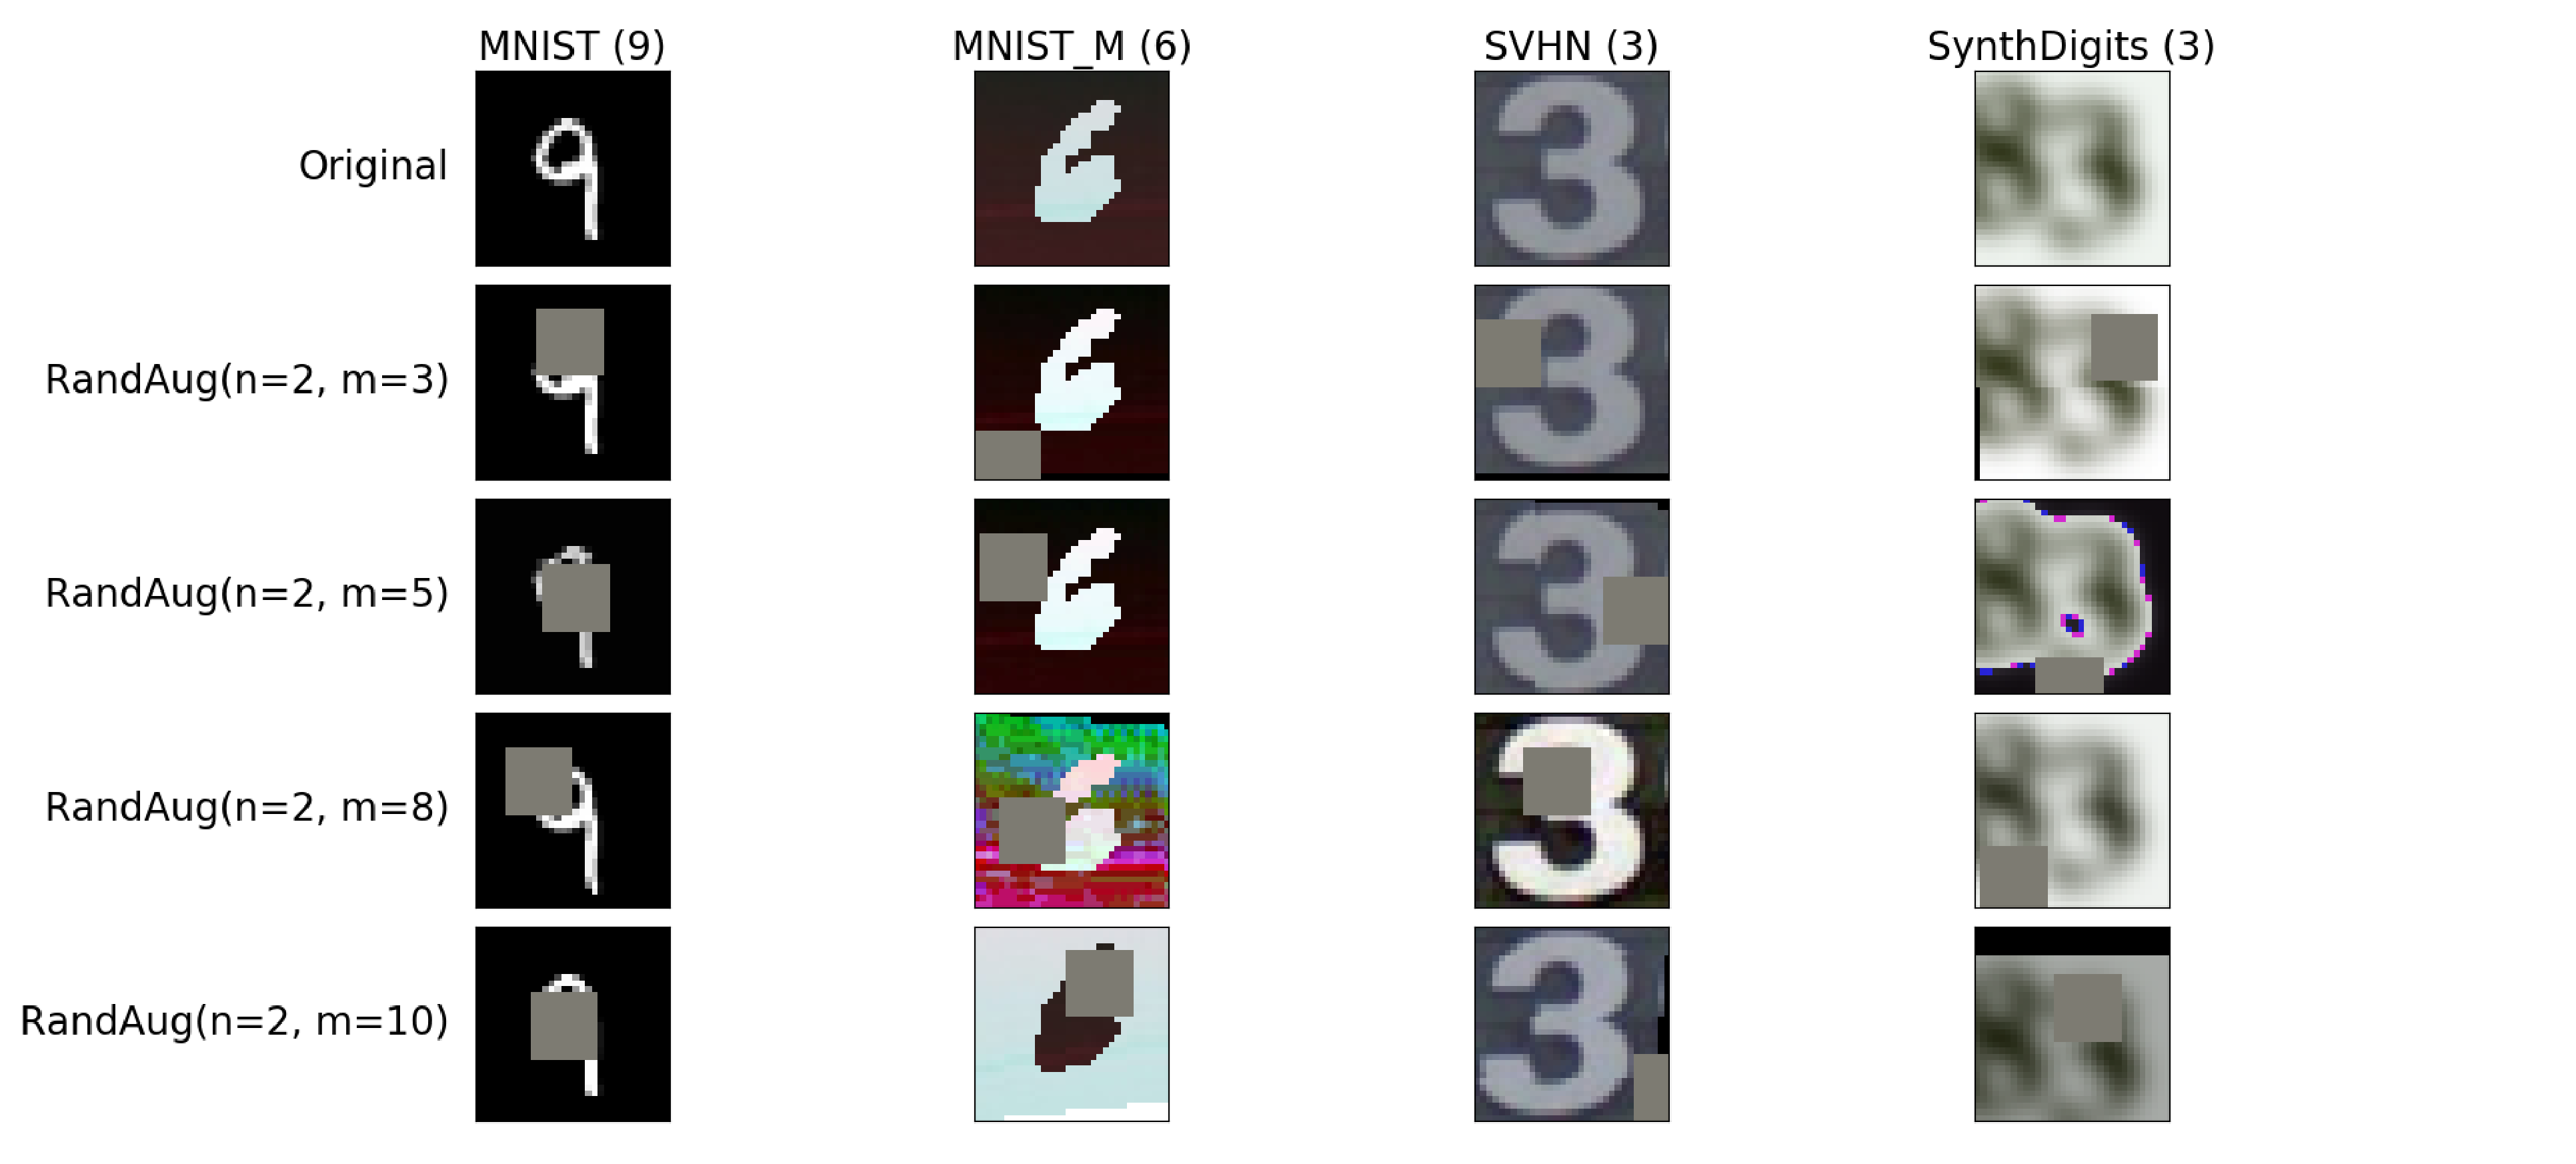
\includegraphics[width=\linewidth]{ChapterThree/digits}
	\caption{Sample original and transformed images from the digits datasets. The ground-truth label is in brackets.}
	\label{fig:digits_samples}
\end{figure}
\begin{figure}[h!]
	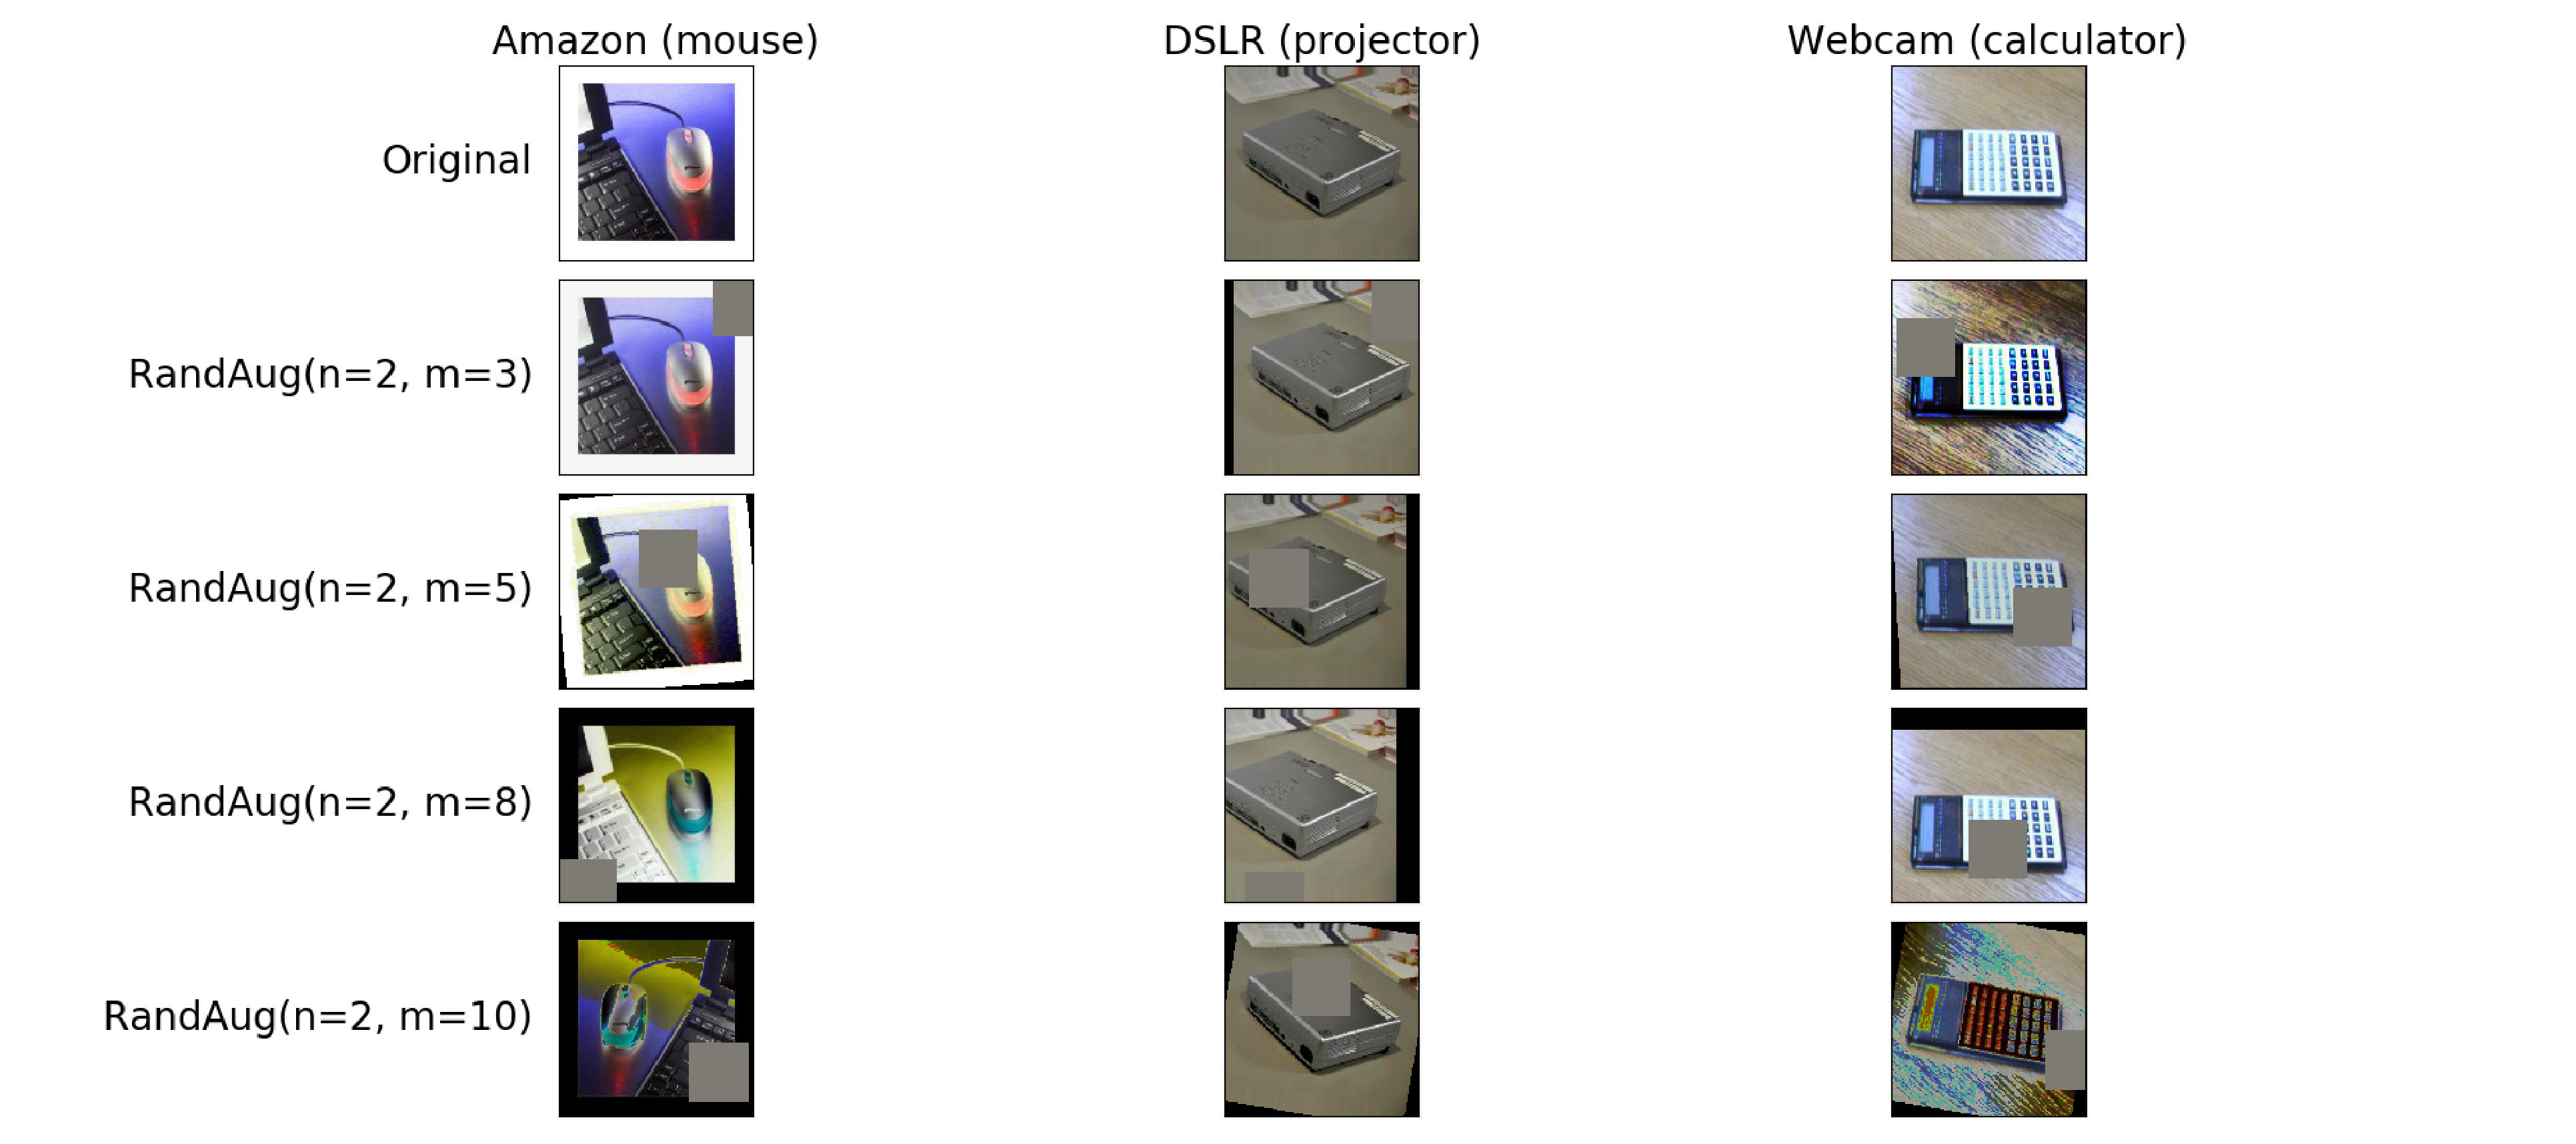
\includegraphics[width=\linewidth]{ChapterThree/office}
	\caption{Sample original and transformed images from each domain in the Office-31 dataset. The ground-truth label is in brackets.}
	\label{fig:office_samples}
\end{figure}
\begin{figure}[h!]
	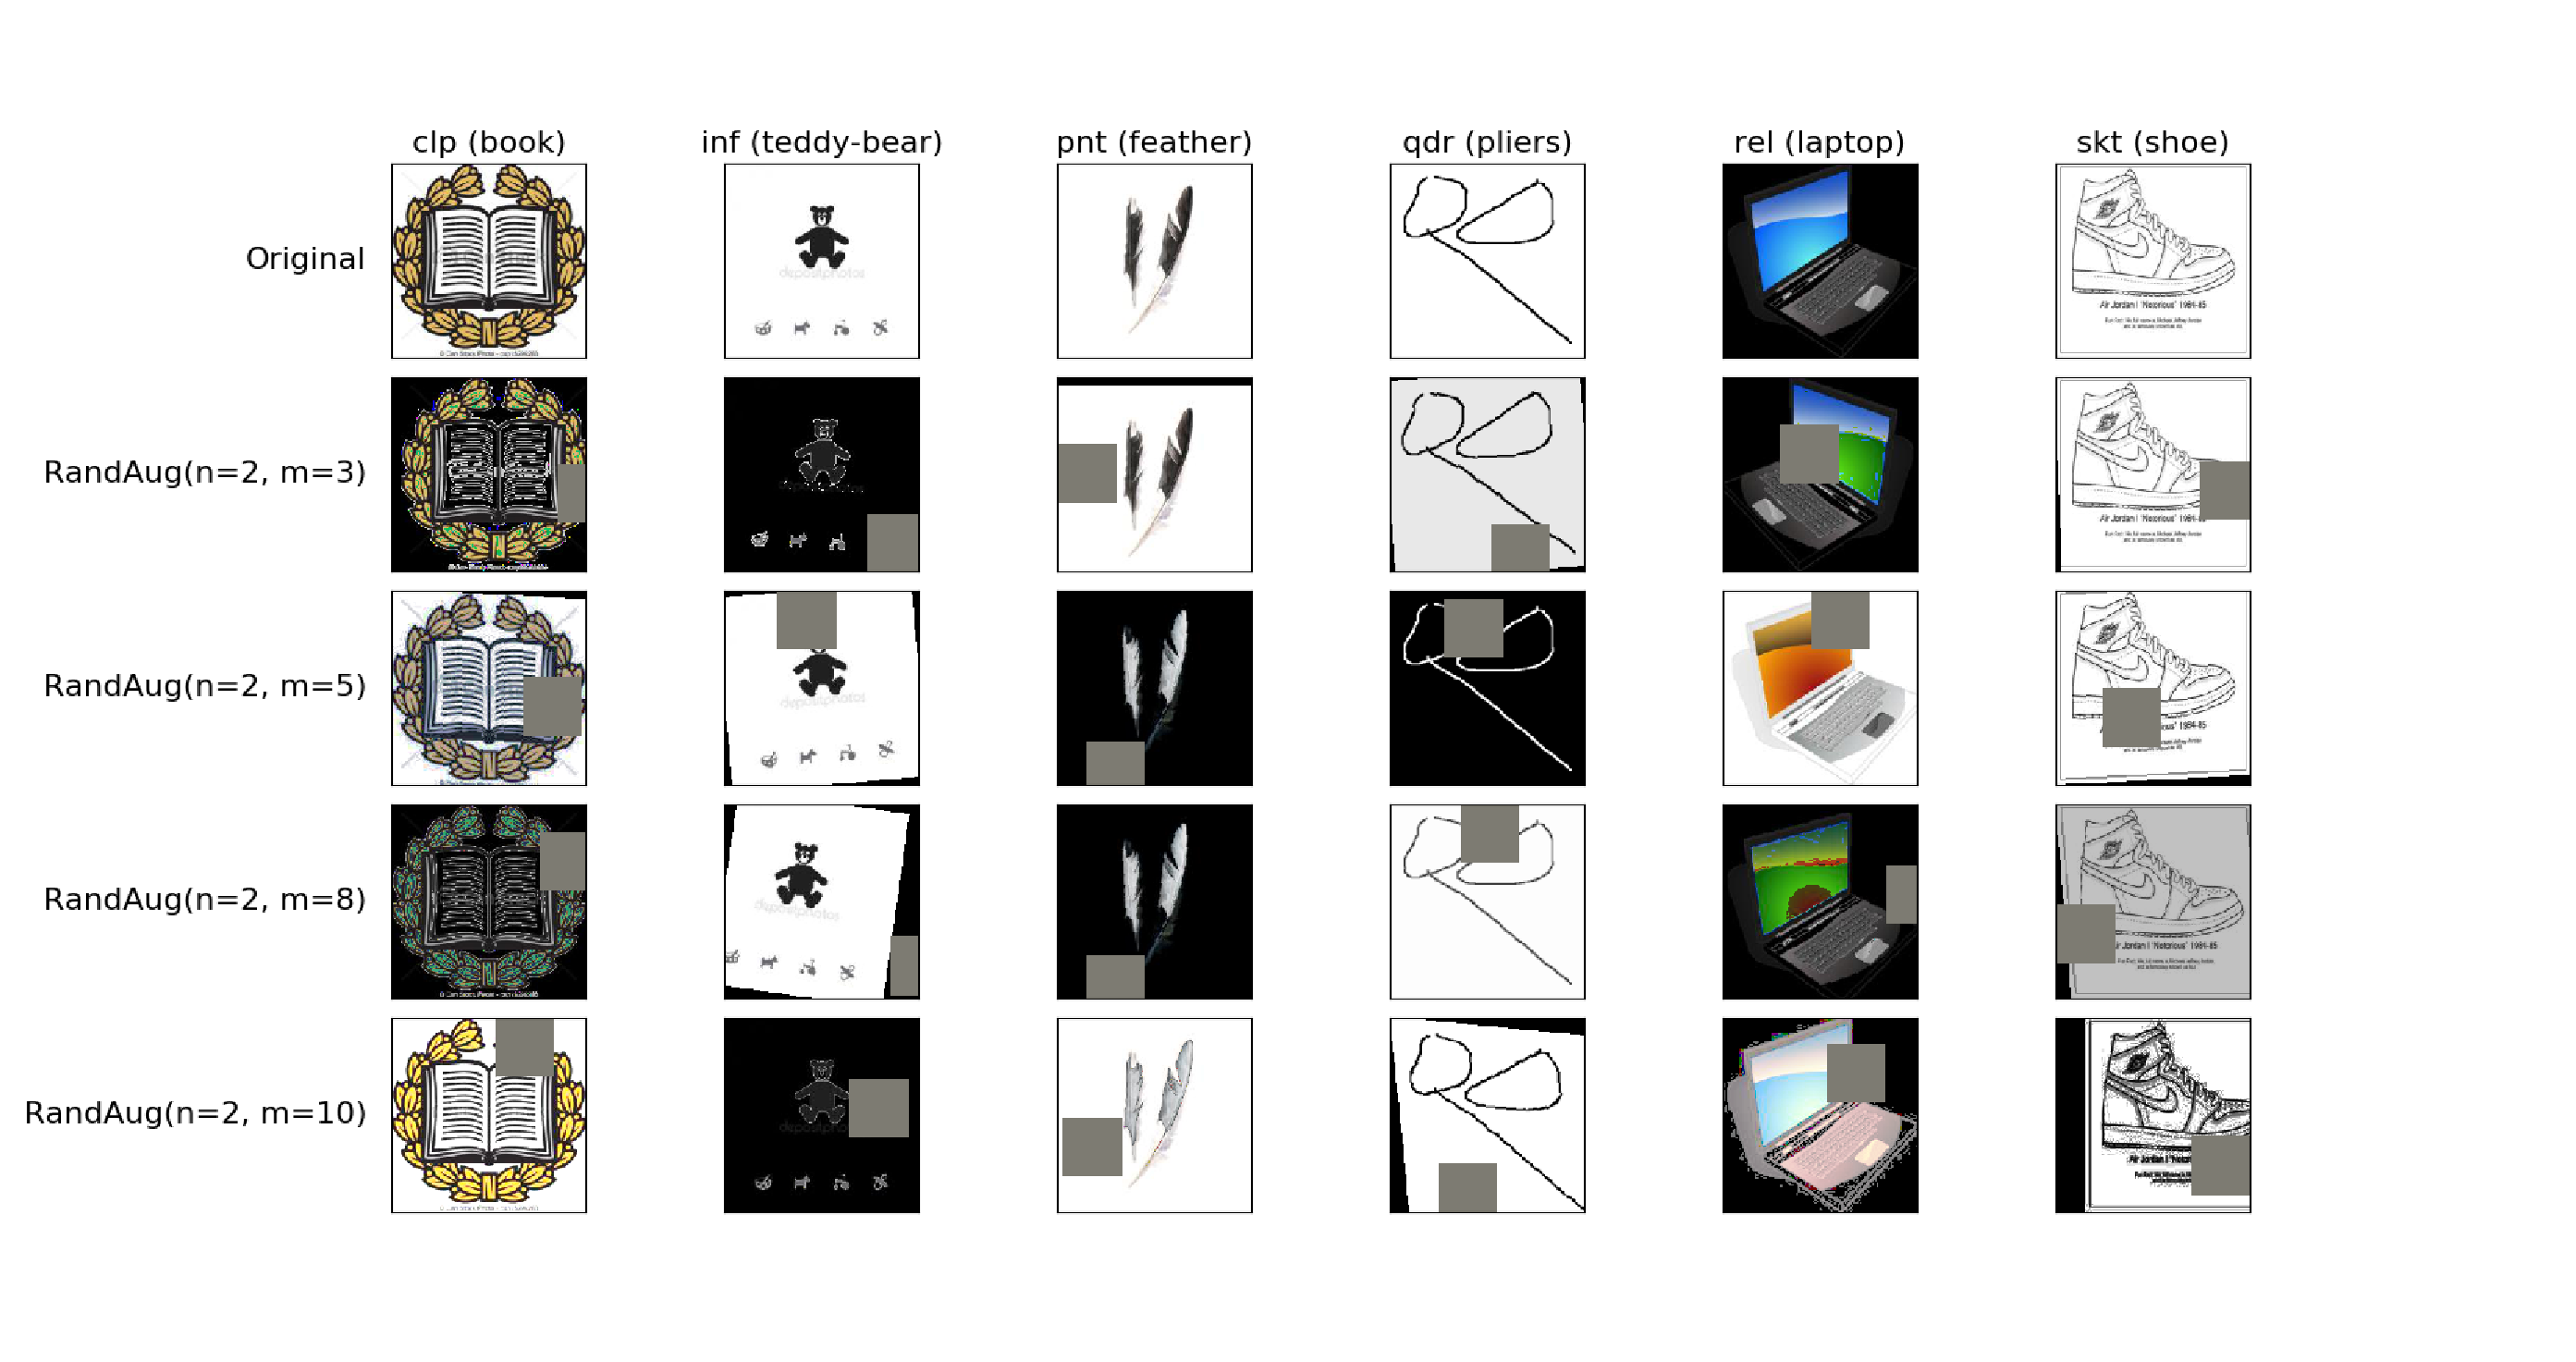
\includegraphics[width=\linewidth]{ChapterThree/domainnet}
	\caption{Sample original and transformed images from each domain in the DomainNet dataset. The ground-truth label is in brackets.}
	\label{fig:domainnet_samples}
\end{figure}
